\documentclass[msc,numbers]{coppe}
\usepackage[utf8]{inputenc}
\usepackage{amsmath,amssymb}
\usepackage{hyperref}
\usepackage{setspace}
\usepackage{caption}
\usepackage{subcaption}
\usepackage{booktabs}
\usepackage{float}
\usepackage{multirow}
\usepackage[table]{xcolor}
\usepackage{indentfirst}
\usepackage{rotating}


\definecolor{lightgray}{rgb}{0.9,0.9,0.9}

\makelosymbols
\makeloabbreviations

\begin{document}
  \title{Identificação de Eventos Baseada na Combinação de Detectores de Altas
  Energias com Diferentes Tecnologias e Segmentações}
  \foreigntitle{Event Identification Based on the Combination of High Energy
  Detectors with Different Technologies and Segmentations}
  \author{Fernando Guimarães}{Ferreira}
  \advisor{Prof.}{José Manoel de}{Seixas}{D.Sc.}

  \examiner{Prof.}{José Manoel de Seixas}{D.Sc.}
  \examiner{Prof.}{Mariane Rembold Petraglia}{Ph.D.}
  \examiner{Prof.}{Amauri Oliveira}{D.Sc.}
  \examiner{Prof.}{André Massafferri Rodrigues}{Ph.D.}
  \department{PEE}
  \date{12}{2012}

  \keyword{Detecção de Partículas}
  \keyword{Física de altas energias}
  \keyword{Redes Neurais}

  \maketitle

  \frontmatter
  \dedication{À memória da Vó Marly.}


  \chapter*{Agradecimentos}


Primeiramente, gostaria de agradecer aos meus pais, Luiza e João, por todo o
apoio. Obrigado por terem me incentivado a buscar meus objetivos.  Agradeço por
todos os conselhos, pela força  e pelos ensinamentos ao longo desta caminhada.

Agradeço também à minha irmã, Ana Luíza, pelo carinho e confiança. Sua
determinação é um exemplo para mim.

Aos meus avós, minha dinda e meus primos que, mesmo distantes, nunca deixaram de
participar de alguma forma.

Ao meu orientador José Manoel de Seixas pela confiança, pelas oportunidades e
todo o suporte dado ao longo desse trabalho.

À Carmen Maidantchik pelas sugestões, pelos conselhos e pela constante
orientação desde os tempos de graduação.

À Ana Henriques pela idealização deste projeto. Agradeço também pela confiança
e por viabilizar a minha participação junto à colaboração \emph{TileCal}.

Ao amigo Thiago Ciodaro por facilitar meu trabalho e encurtar o tempo de
aprendizado sobre múons e afins, compartilhando seu conhecimento com muita
paciência.

Aos amigos e sócios da TWIST: Andressa Sivolella\footnote{Agradecimento
especial pela grande ajuda na revisão deste documento}, Felipe Grael, Laura
Moraes e Luiz Évora. Agradeço por compartilharem da mesma motivação e pelo
companherismo cotidiano.

À colaboração e amizades de todos no TileCal/CERN, que desde 2007 fazem de
Genebra um lugar especial. Agradeço principalmente: Carlos,
Giorgi, Brian, James, Heuijin, Keith, Gabriel, Filipe, Luis, Denis, Rob, Ali,
Jalal, Stan, Irene, Monica,  David e, claro, Bob Stanek.

Aos brasileiros ``genebrinos'' que também participaram de alguma forma ao longo
desta jornada: Bruno Carneiro, Bernardo, Denis, Torres, Dhiana, Júnior, Enoque,
Eric, Frias, Bruno Lange. Agradeço a convivência e as histórias decorrentes
dela.

À todos participantes do Projeto TB: Afrânio, Dani, Priscila, Karina,
Faier~(\emph{Finscore}) e Frank~(\emph{Finscore}) que enriqueceram minha
experiência neste período de Mestrado das mais diversas maneiras.

Por fim, agradeço a todos meus amigos pelo invariável apoio e por todos os
momentos de descontração.




  \begin{abstract}

O CERN localiza-se na fronteira entre a Suíça e a França, próximo a cidade de
Genebra. Nele opera o LHC, o maior e mais poderoso acelerador de partículas do
mundo. No LHC, pacotes de prótons são injetados e acelerados até a energia
aumentar 15 vezes, adquirindo 7~TeV. Os objetivos do projeto demandam uma
elevada taxa de tomada de dados. Assim, o LHC opera a 40~MHz. Operando na
luminosidade máxima projetada para o colisor, a taxa de eventos poderá alcançar
1~GHz. Desta maneira, torna-se fundamental a realização de uma filtragem
\emph{online}, onde informações relevantes são extraídas do ruído de fundo com
velocidade condizente a taxa de dados gerados.

A identificação de múons de todos os patamares energéticos é crucial para
explorar todo potencial físico disponível através da operação do ATLAS. Através
da observação destas partículas é possível conhecer novas físicas. O
Espectrômetro de Múons é instalado na área externa do ATLAS e foi projetado para
detectar essas partículas.  Contudo, há regiões onde não há cobertura total de
estações. Nestas áreas todos os múons são classificados automaticamente como
pouco energéticos, prejudicando a eficiência de detecção.

Esta dissertação utiliza técnicas de processamento de sinais e
inteligência computacional para auxiliar o primeiro nível de filtragem a
recuperar múons com alto valor de momento transverso, erroneamente classificados.
\end{abstract}


  \begin{foreignabstract}

CERN is located in the border between Switzerland and France, near to Geneva
city. The LHC is operating there. It's is the world's largest and most powerful
particle acellerator. In the LHC, protons packages are injected and acellerated
until its energy increases by 15 times, summing up 7~TeV. The project goals
require enormous data acquisition rates. Therefore, the LHC has a peak crossing
rate of 40~MHz. The event rate can get up to 1~GHz after the upgrade that will
start next year. This way, it's crucial to filter online where only relevant
information is observed against the background noise within the processing speed
requirements.

The muon identification is very important for exploring the entire physics
potential available with the ATLAS operation. It is possible to observe new
physics through the observation of such particles. The Muon Spectrometer is
installed on the ATLAS' surrond and it was designed to detect this elements.
However, some of the detector's region are not covered by its trigger stations.
In this areas, every muon is qualified as a low $p_T$ one, harming the detection
performance.

This M.Sc. project use signal processing and computing intelligence techniques
for aiding the Level-1 trigger to recover these muons with high transverse momentum.

\end{foreignabstract}


  \tableofcontents
  \listoffigures
  \listoftables
  \printlosymbols
  \printloabbreviations

  \mainmatter
  \begin{spacing}{1.5}
  \chapter{Introdução}

A evolução e o desenvolvimento de técnicas de processamento de sinais e
inteligência computacional impulsionam diversas áreas do conhecimento. Pode-se
observar uma infinidade de aplicações nos mais diversos segmentos. Tais
ferramentas tendem a se tornar ainda mais poderosas quando utilizadas juntas.
Esta multidisciplinaridade característica, somada às inúmeras possibilidades de
abordagem de um problema, tornam a pesquisa nessas áreas instigante.

Este trabalho de pesquisa acontece no âmbito da detecção de sinais em ambientes
com baixa relação sinal-ruído. Experimentos dessa natureza apresentam um grande
volume de informações e elevadas dimensões em seu espaço amostral, dificultando
o processo de análise. A taxa de eventos tende a ser muito
elevada, pelo caráter raro dos sinais de interesse. Desta maneira, torna-se
fundamental a realização de uma filtragem \emph{online}, onde informações
relevantes são extraídas do ruído de fundo com velocidade condizente a taxa de
dados gerados.

Dependendo da aplicação, a aquisição de dados pode envolver detectores com
diferentes segmentações, contando com diversos sensores e canais, muitas vezes
distintos entre si.  Como consequência, são necessários sistemas robustos com
baixo custo computacional para contornar todas as condições hostis do projeto
especificado.

\section{Motivação}

A física experimental de altas energias é um dos ramos da ciência onde as
técnicas de processamento de sinais e inteligência computacional são mais
exigidas. Nela, procura-se comprovar experimentalmente teorias propostas pela
física teórica. Para tal, são construídos aparatos de proporções,
capazes de criar as condições ideais para a obtenção da física de interesse.

O LHC, instalado no CERN, é um acelerador capaz de atingir níveis de energia
nunca antes alcançados. O ATLAS, o maior dos detectores do acelerador, possui
milhões de canais de leitura, distribuídos por diferentes subsistemas,
utilizados para identificar partículas geradas com as colisões ocorridas durante
a operação.

Partindo do ponto de colisão em direção a área externa do ATLAS, encontram-se o
Detector de traços, utilizado para a identificação da trajetória de determinadas
partículas; o Calorímetro Eletromagnético e o Calorímetro Hadrônico, para a
análise da deposição energética de partículas eletromagnéticas e hadrônicas,
respectivamente; e o Espectrômetro de Múons, para a identificação
e determinação da trajetória de múons.

No ATLAS, ocorrem quarenta milhões de eventos por segundo, onde apenas duzentos
serão selecionados e armazenados para uma posterior análise \emph{offline}.
Deste modo, um sistema \emph{online} de filtragem eficiente é indispensável.
Esta seleção ocorre em 3 etapas através de níveis sequenciais:

\begin{enumerate}

    \item O primeiro nível do sistema de filtragem recebe todos os eventos
    gerados nas colisões. Neste ponto, apenas um em aproximadamente quinhentos e
    quarenta eventos é aceito.  A seleção é realizada através de \emph{hardware}
    de baixa granularidade utilizando informações de baixa resolução do sistema
    de calorimetria e do detector de múons, o que garante a velocidade de
    processamento necessária.

    Este nível também é responsável por gerar as chamadas Regiões de Interesse,
    áreas onde há informação relevante. Estas regiões são propagadas para o
    segundo nível;

    \item O segundo nível de filtragem considera apenas as regiões de interesse
    selecionadas na etapa anterior. Para tal, os algoritmos de filtragem têm
    acesso a resolução máxima do detector, bem como a trajetória percorrida
    pelas partículas.

    \item O terceiro nível de filtragem, conhecido como \emph{Event Filter},
    utiliza toda a informação adquirida para um evento. Ele é capaz de combinar
    as diferentes regiões de interesse para reconstruir os processos físicos
    ocorridos após a colisão.
\end{enumerate}

Com o advento do \emph{upgrade} do detector, previsto para a operação em 2020,
com etapas intermediárias em 2013 e 2017, novas arquiteturas podem ser propostas
e testadas~\cite{TSENG2008}.

\section{Objetivo}

Este trabalho de pesquisa utiliza técnicas de processamento de sinais e
inteligência computacional para auxiliar o primeiro nível de filtragem na
identificação de múons com alto valor de momento transverso.

Múons são partículas, eletricamente carregadas, duzentas vezes mais pesadas do
que os elétrons. Sua  identificação é crucial para explorar todo potencial
físico disponível através da operação do ATLAS. São de interesse do experimento
múons com poucos GeV até elevados patamares energéticos, onde é possível a
identificação de Nova Física~\cite{HASSANI2007}.

O Espectrômetro de Múons é instalado na camada externado ATLAS. Foi projetado
para detectar e reconstruir a trajetória de partículas que transpassam pelos
sistemas de calorimetria.

Por ser muito pesado, o múon dissipa pouca energia ao cruzar os detectores que
estejam ao longo de seu caminho. A estratégia do sistema de múons é aplicar um
campo magnético intenso, capaz de curvar a trajetória da partícula.  O múon
atravessará três camadas, compostas por câmaras resistivas,  ao longo de seu
percurso.  A posição em que a partícula cruza cada uma destas camadas determina
a curvatura de sua trajetória, que por sua vez é utilizada na determinação do
valor do momento linear. Quanto maior a energia cinética da partícula mais
suave será o seu raio de curvatura. Desta forma, entende-se que múons mais
energéticos obrigatoriamente atravessam as três camadas (ou estações de
coincidência) do espectrômetro, enquanto as menores podem passar apenas por
duas, devido ao desvio proporcionado pelo campo magnético aplicado. Este é,
portanto, um critério para distinção entre múons de alto momento e de baixo
momento.

Contudo, há regiões onde não há cobertura de câmaras nas três camadas. Nestas
áreas todos os múons são classificados automaticamente como pouco energéticos,
prejudicando a eficiência~\cite{ATLAS-CONF-2012-099}.

O Calorímetro de Telhas, por sua vez, é segmentado radialmente em três camadas.
Nelas, partículas hadrônicas, tais como prótons, são absorvidas. Contudo, em
virtude da espessura deste detector, a terceira camada possui baixa atividade de
interações com estas partículas, pois a maioria já foi absorvida nas duas
camadas mais internas. É nesta região que se localizam as chamadas células D.
Entende-se que as informações adquiridas nestas células  possam ser utilizadas
para mitigar o ruído de fundo na aquisição de múons.

Este trabalho utilizou as informações geométricas do calorímetro e do sistema de
múons, somadas a energia depositada pela passagem de partículas na célula D para
recuperar múons de momento elevado que não tiveram sua passagem registrada nas
três estações de coincidência.

\section{Organização do documento}

O próximo capítulo apresenta uma visão geral do ambiente do CERN, do experimento
ATLAS e seus sub-detectores.  O capítulo 2 apresenta mais detalhadamente o
Calorímetro de Telhas e o Espectrômetro de Múons, pois a presente pesquisa foi
desenvolvida no âmbito dos dois sistemas.  O Capítulo 3 apresenta o sistema de
seleção de partículas do ATLAS. O nível 1 de filtragem, que utiliza informações
da calorimetria e do sistema de múons em seus algoritmos, é explicado em
detalhes. O Capítulo 4 mostra a base de dados utilizada para realizar as
análises e as diferentes abordagens adotadas. O Capítulo~5  é dedicado para a
apresentação e discussão dos resultados obtidos.   Por fim, as conclusões, bem
como os possíveis desdobramentos deste trabalho de pesquisa, são apresentados no
Capítulo~6.

  \chapter{CERN, LHC e o Experimento ATLAS}

A Ciência procura compreender as leis que regem a Natureza. Uma das questões
mais antigas desta busca refere-se à constituição da matéria. A Física de
Partículas é a parte da física que estuda os constituintes da matéria e as
interações entre eles.

A matéria como conhecemos é formada por partículas estáveis. Há, porém,
partículas instáveis que duram apenas frações de segundos. Ambos tipos
coexistiram nos instantes posteriores ao \emph{Big Bang}.

É possível observar essas partículas instáveis utilizando os aceleradores de
partículas. Nesses aparelhos, um feixe de partículas, como prótons ou elétrons,
são aceleradas até altas velocidades, aumentando a energia cinética.  Quando a
energia chega ao patamar desejado, o feixe é colidido com outro grupo de
partículas, recriando assim as condições ideais para a formação de partículas
instáveis.

O CERN~(\emph{Organisation européenne pour la recherche nucléaire}) é o maior
laboratório de física de partículas do mundo e nele se encontra o mais complexo
aparato científico já construído pelo homem, o LHC~(\emph{Large Hadron
Collider})~\cite{EVANS2008}. Neste capítulo será apresentado este acelerador,
com enfoque no detector ATLAS e seus subsistemas.

\section{Breve Introdução ao Modelo Padrão}

O modelo atômico de Rutherford-Bohr, apresentado em 1913, é amplamente
conhecido. Nele prótons, nêutrons e elétrons são os componentes básicos dos
átomos. Esta noção é correta, porém existem partículas ainda menores. Hoje
sabe-se que tudo é formado pela combinação de 16 elementos fundamentais:
\emph{quarks}, \emph{léptons} e os transportadores de força (ou \emph{bósons}).
O Modelo Padrão, publicado no final da década de 1960, explica a função destas
partículas bem como as que forças atuam sobre elas~\cite{GRIFFITHS2008}. A
Figura~\ref{fig:modelopadrao} apresenta os elementos básicos desse modelo:

\begin{figure}[htpb!]
    \centering
    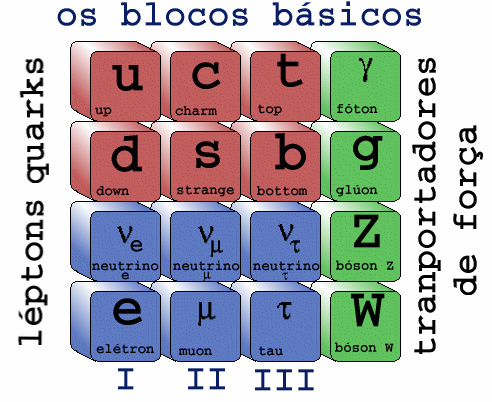
\includegraphics[width=8cm]{images/modelo_padrao.png}
    \caption{Modelo padrão de partículas elementares.}
    \label{fig:modelopadrao}
\end{figure}

Os prótons e nêutrons presentes no núcleo atômico  são compostos por
\emph{quarks}. Existem seis tipos de quarks frequentemente agrupados em duplas:
\emph{up}/\emph{down}, \emph{charm}/\emph{strange}, \emph{top}/\emph{bottom},
todos com seu \emph{anti-quarks} correspondente. \emph{Quarks} nunca são observados
separadamente.

Quando \emph{quarks} se agrupam, formam uma partícula composta chamada hádron.
Hádrons podem ser separados em duas categorias: bárions, formados por até três
\emph{quarks}, e mésons, formados por um \emph{quark} e um \emph{anti-quark}.
Prótons e nêutrons são tipos de bárions.

O Modelo também prevê seis tipos de léptons: elétrons, múons, tau e seus
respectivos neutrinos. Assim como os \emph{quarks} possuem \emph{anti-quarks},
léptons possuem anti-léptons. Contudo, os léptons podem ser observados
isolados. Elétrons, múons e tau são partículas carregadas e possuem massa,
enquanto neutrinos não possuem carga e possuem pouquíssima massa.  O lépton tau
e o múon são extremamente pesados e altamente instáveis. Por isso, decaem
rapidamente em léptons mais leves. Já os elétrons e neutrinos são muito
estáveis, sendo facilmente observados.

Partículas transportadoras de força são mensageiras que carregam uma
discreta quantidade de energia de um elemento para a outro. São elas os fótons, glúons e
os bósons W e Z. Fótons atuam nos \emph{quarks} e carregam léptons, exercendo a força
eletromagnética. Glúons atuam nos \emph{quarks} mantendo-os unidos. Já os bósons
W e Z representam a força-fraca que atua tanto em léptons como em \emph{quarks}.
A única força não esclarecida pelo Modelo Padrão é a gravitacional. Existe a
possibilidade que haja uma partícula graviton, ainda não
observada~\cite{PERKINS2000}.

\section{Organização Europeia para Pesquisa Nuclear}

O CERN localiza-se na fronteira entre a Suíça e a França, próximo a cidade de
Genebra. Foi fundado com o objetivo de criar um laboratório europeu para
pesquisa de física nuclear, em que seus países membros pudessem dividir as
despesas de seus aparatos e instalações. Estimulados pelas diversas organizações
internacionais nascentes na Europa pós-guerra, um grupo de cientistas formaram
um conselho provisório em 1952, base para a fundação da atual organização,
ocorrida dois anos depois~\cite{ACZEL2012}. A Figura~\ref{fig:scienceglobe} mostra o
Globo de Ciências e Inovação, construído na ocasião do quinquagésimo aniversário
de fundação do CERN.

Atualmente, o CERN é dirigido por 20 Estados membros europeus (a
Figura~\ref{fig:cernflags} representa as respectivas bandeiras localizadas sua
entrada principal do instituto).  Contudo, outros países não-membros colaboram
das mais diversas maneiras, inclusive o Brasil.  No total, existem cerca de
8.000 cientistas provenientes de 608 universidades, representando 113
nacionalidades~\cite{ref:cern_www}.

\begin{figure}[htpb!]
        \centering
        \begin{subfigure}[b]{0.45\textwidth}
                \centering
                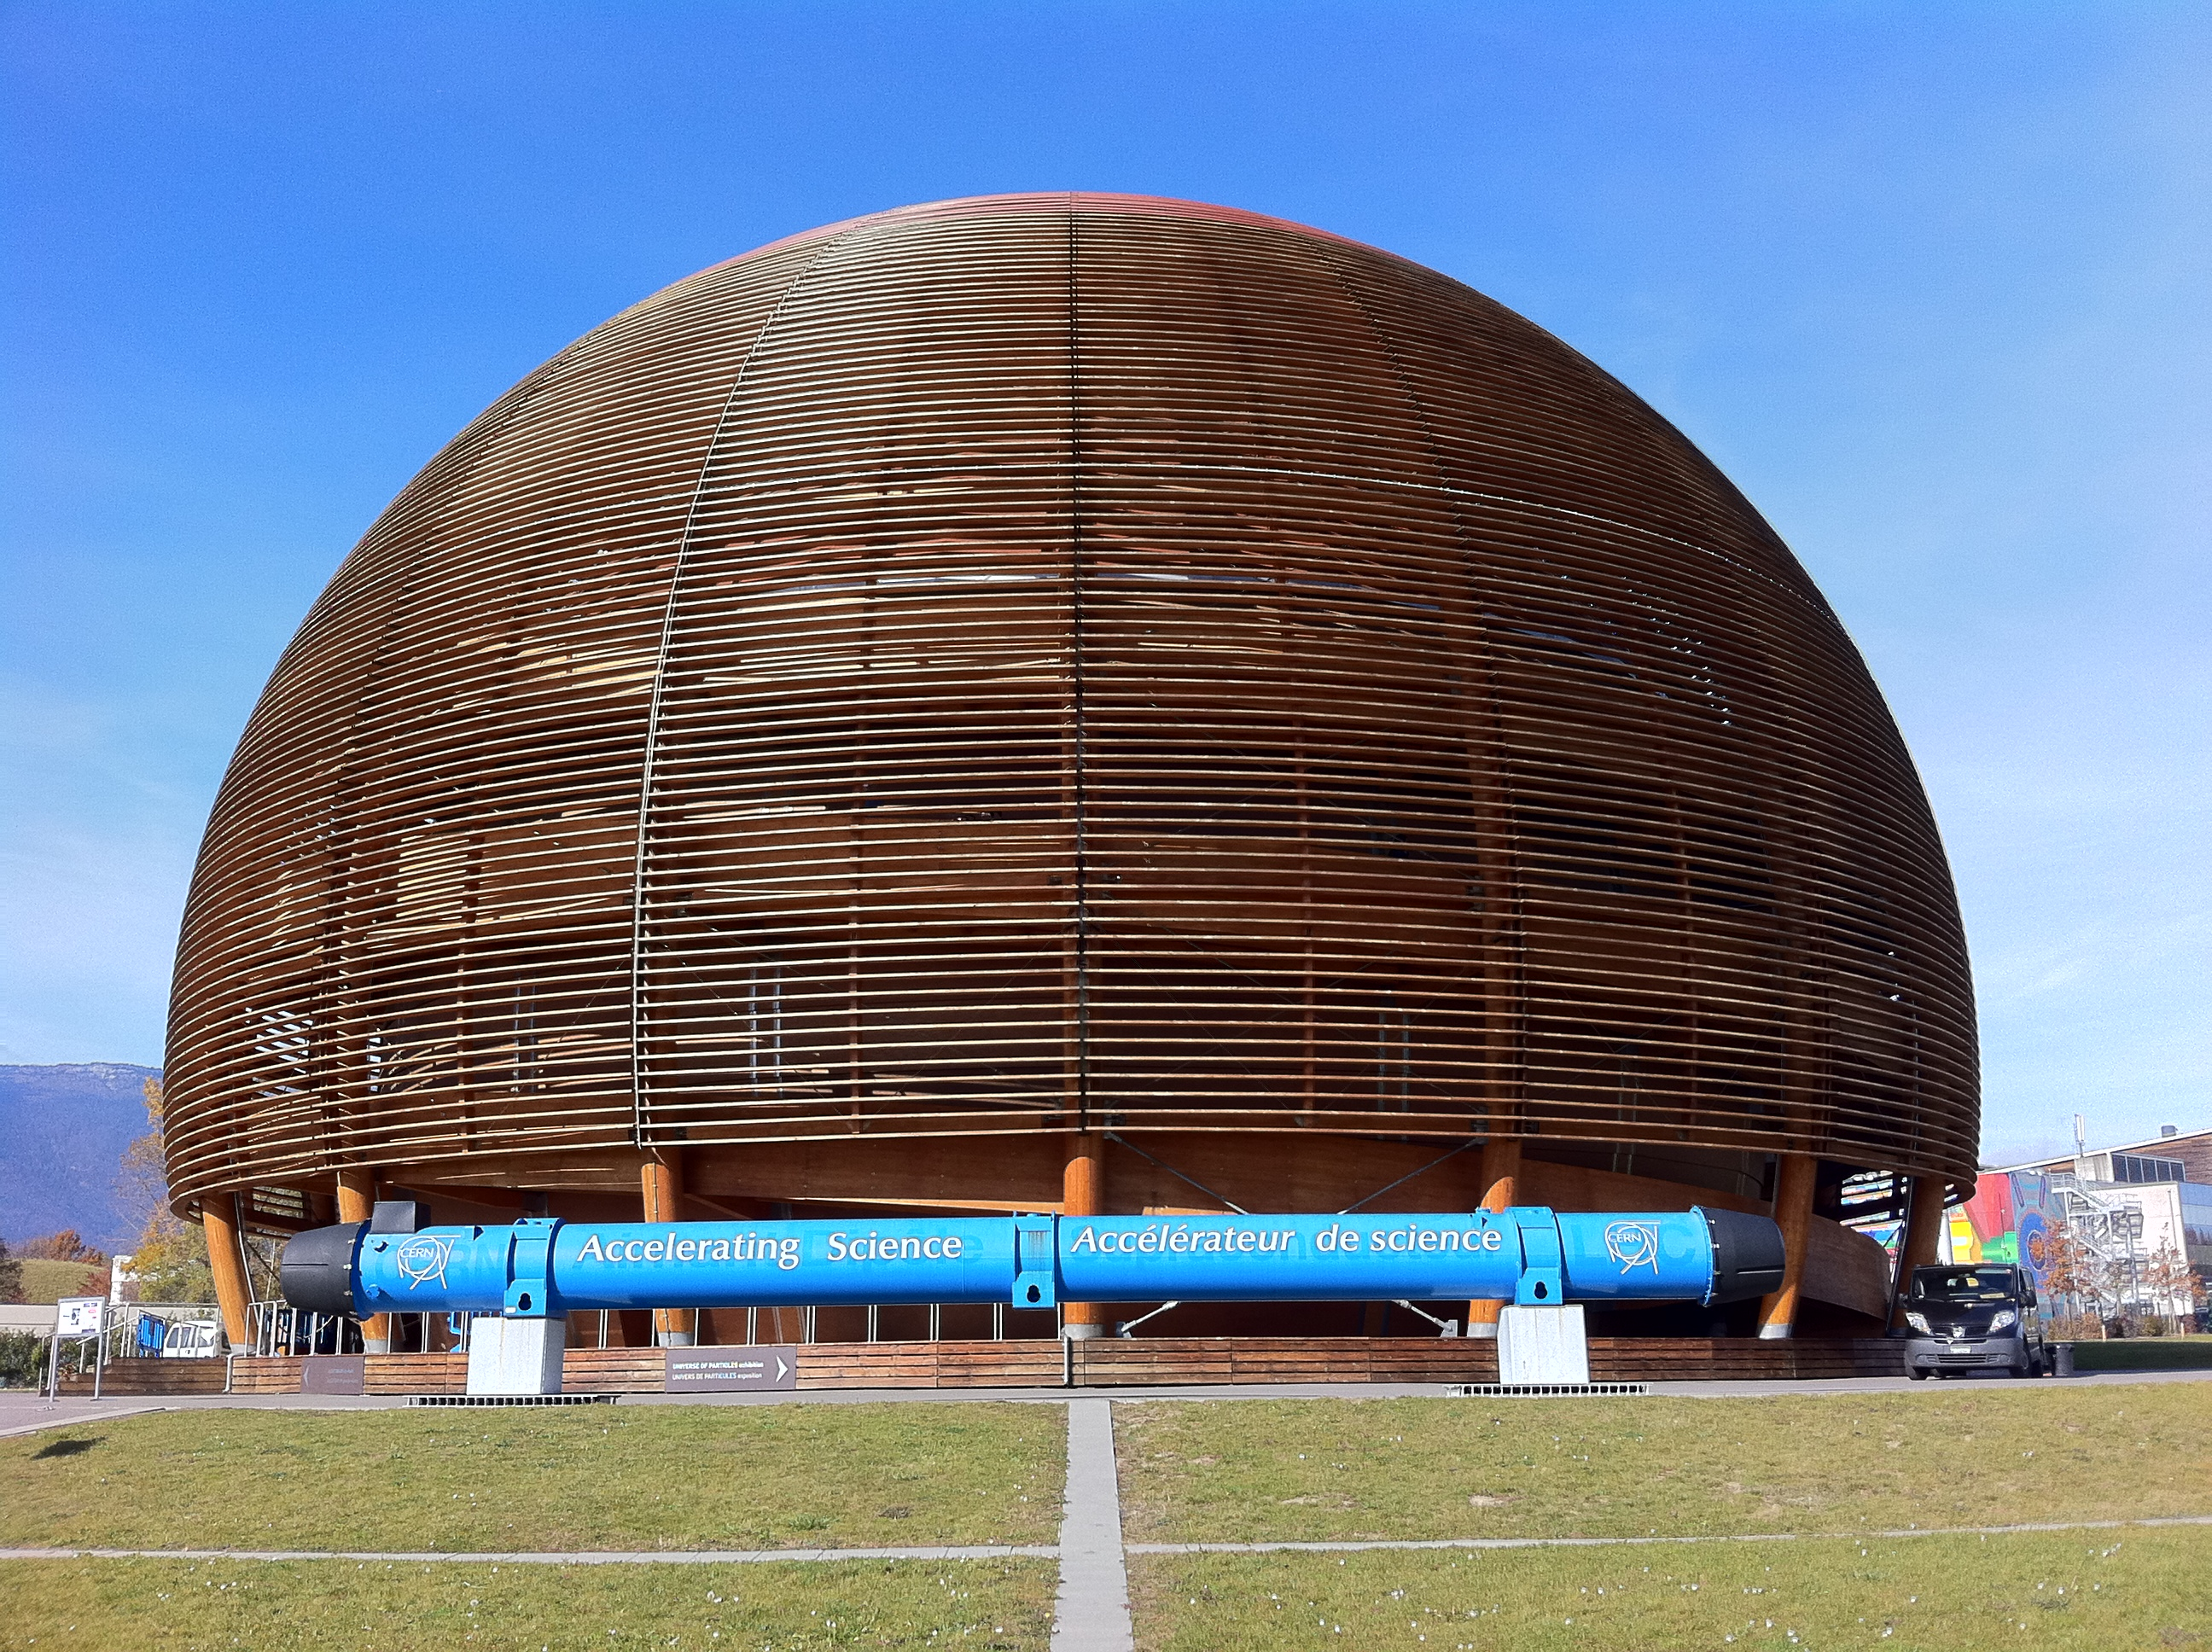
\includegraphics[trim=0cm 4cm 0cm 3cm, clip=true,width=\textwidth]{images/innovation_globe.jpg}
                \caption{ O Globo da Ciência e Inovação do CERN.}
                \label{fig:scienceglobe}
        \end{subfigure}%
        ~
        \begin{subfigure}[b]{0.45\textwidth}
                \centering
                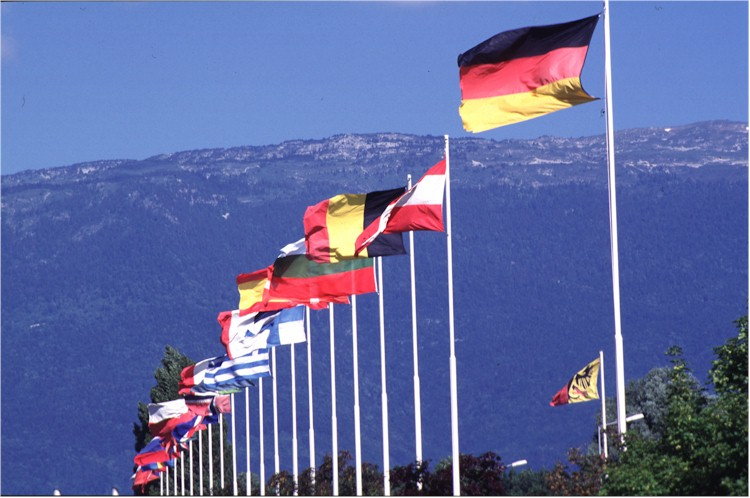
\includegraphics[width=\textwidth]{images/cern_flags.jpg}
                \caption{ Bandeiras dos países membros da organização.}
                \label{fig:cernflags}
        \end{subfigure}
        \caption[Fotografias de marcos no CERN.]{CERN: O maior laboratório de
        pesquisa nuclear do
        mundo (Imagens extraídas de~\cite{ref:cern_www}).}\label{fig:cern1}
\end{figure}

Além da colaboração à comunidade de física de partículas, o CERN contribui com
o desenvolvimento de tecnologias empregadas em diversas áreas. A invenção
da~\emph{World Wide Web}, equipamentos de imagens medicinais e a computação em
GRID são apenas alguns dos exemplos.

\section{O Projeto LHC (~\emph{Large Hadron Collider})}

O LHC, o maior e mais poderoso acelerador de partículas do mundo, é o mais novo
aparato do complexo de aceleradores do CERN (Figura~\ref{fig:cerncomplex}). Ele
foi construído no túnel onde o LEP~\cite{ref:PICASSO1990} operou entre 1989 e
2000.  Esse túnel possui uma circunferência de 27~km de extensão e está
posicionado 150 metros abaixo da superfície. A Figura~\ref{fig:lhc} apresenta
um esquemático do anel do LHC e os principais experimentos localizados nele.

\begin{figure}[htpb!]
    \centering
    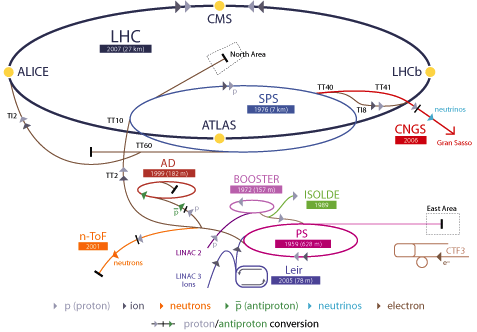
\includegraphics[width=12cm]{images/complexo_acelerador_CERN.png}
    \caption[Complexo de aceleradores no CERN.]{Complexo de aceleradores no CERN
    (Extraído de~\cite{ref:solans}).}
    \label{fig:cerncomplex}
\end{figure}

Antes de serem injetados com uma energia de 450~GeV no anel do LHC, prótons são
acelerados formando feixes. Esses feixes são acelerados até a energia
aumentar 15 vezes, adquirindo 7000~GeV~\cite{ref:solans}. Quando essa energia é
atingida, os feixes são colididos nos centro dos experimentos presentes ao longo
da trajetória. As colisões do LHC possuem energia no centro de massa de 14TeV e
uma luminosidade projetada  de $10^{34}~cm^{-2}s^{-1}$.

O objetivo do projeto demanda uma elevada taxa de tomada de dados. O LHC opera a
40~MHz, ou seja, há a injeção de feixes a cada 25~ns. Operando na luminosidade
máxima projetada para o colisor, a taxa de eventos poderá alcançar
1~GHz~\cite{EVANS2008}.

\begin{figure}[htpb!]
    \centering
    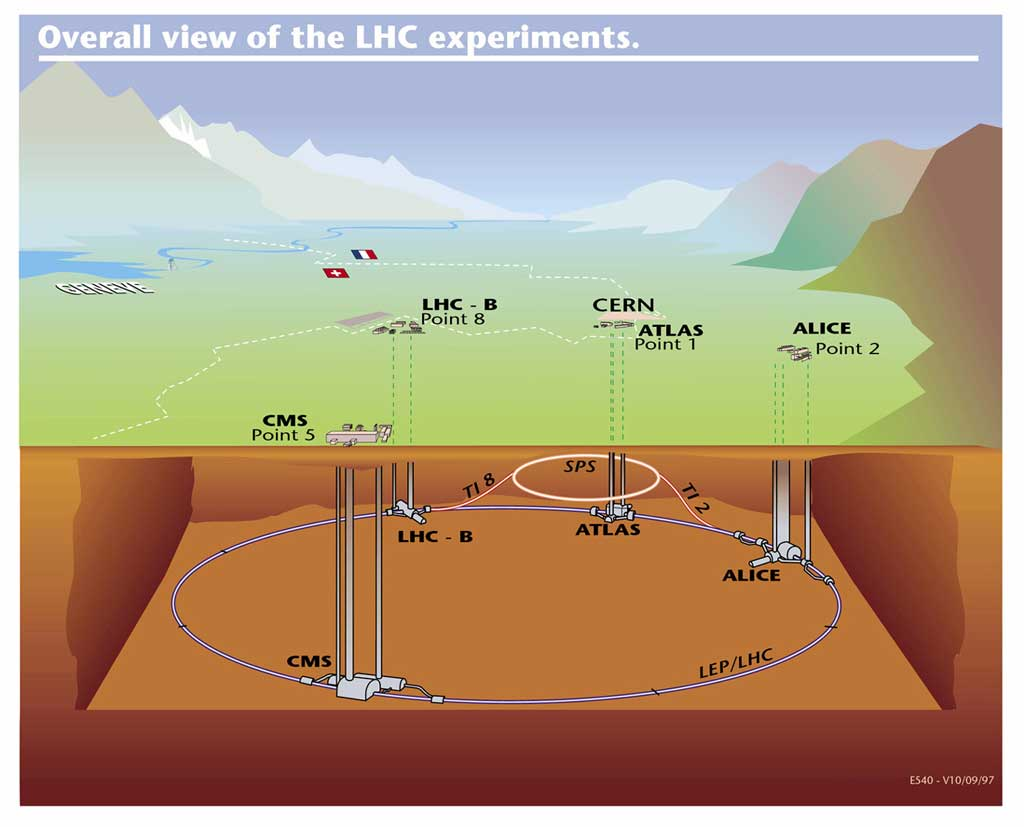
\includegraphics[width=10cm]{images/lhc-sim.png}
    \caption[Diagrama esquemático do túnel do LHC.]{Diagrama esquemático do
    túnel do LHC (Extraído de~\cite{ref:cern_www}).}
    \label{fig:lhc}
\end{figure}

O LHC começou a funcionar em 10 de setembro de 2008. Houve, porém, um acidente
que interrompeu sua operação. Apenas em 2009, as atividades foram retomadas com
a energia de centro de massa de $\sqrt{s} = 3,5~TeV$. Em 2010, colisões com a
metade da energia projetada foram obtidas. A operação ocorre de forma contínua
até  2013, quando ocorrerá um grande período de manutenção e a primeira fase de
atualização dos equipamentos~\cite{ref:ANDERSON2011}.

\subsection{Os experimentos do LHC}

Quatro grandes experimentos estão localizados ao redor da circunferência do LHC,
como foi mostrado na Figura~\ref{fig:lhc}: ATLAS~\cite{ATLAS2008, ref:BOELAERT2012},
CMS~\cite{ref:CMS}, LHCb~\cite{ref:SZUMLAK2010} e ALICE~\cite{ref:ALICE2008}. A
Figura~\ref{fig:experiments} ilustra os experimentos.


\begin{figure}[h!]
    \centering
    \begin{subfigure}[b]{0.45\textwidth}
        \centering
        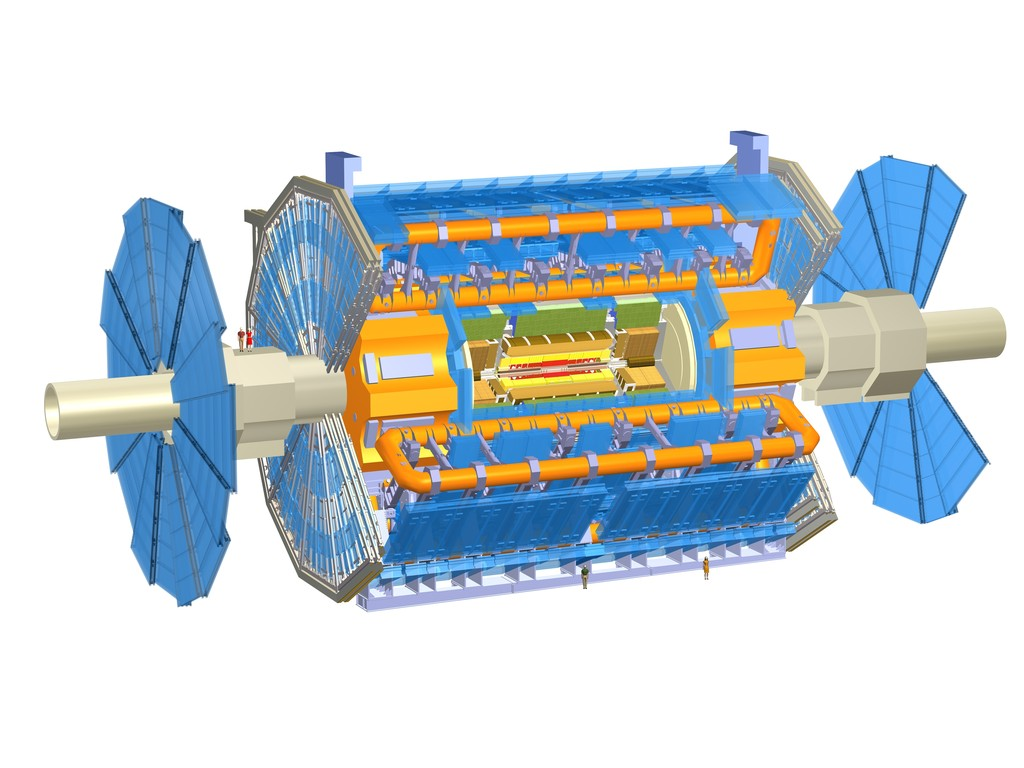
\includegraphics[width=\textwidth]{images/ATLAS.jpg}
        \caption{ATLAS}
    \end{subfigure}%
    ~
    \begin{subfigure}[b]{0.45\textwidth}
        \centering
        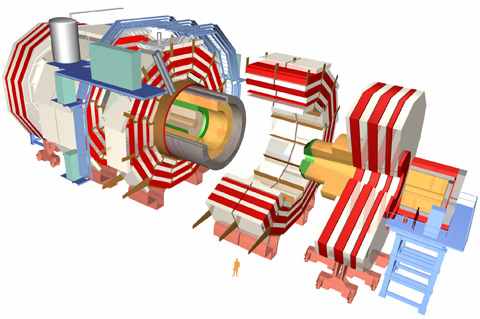
\includegraphics[width=\textwidth]{images/cms.jpg}
        \caption{ CMS}
    \end{subfigure}
    \\
    \begin{subfigure}[b]{0.45\textwidth}
        \centering
        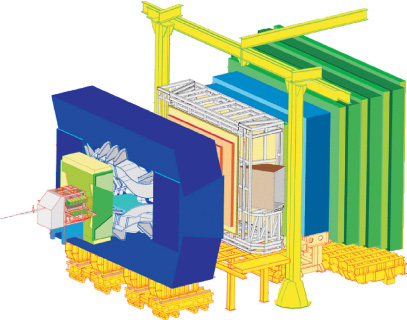
\includegraphics[width=\textwidth]{images/lhcb.jpg}
        \caption{LHCb}
    \end{subfigure}
    ~
    \begin{subfigure}[b]{0.45\textwidth}
        \centering
        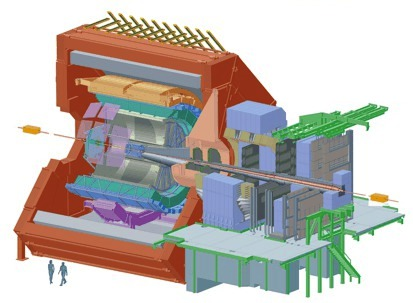
\includegraphics[width=\textwidth]{images/alice.jpg}
        \caption{ ALICE}
    \end{subfigure}
    \caption[Os quatro principais experimentos do LHCb]{Os quatro principais
    experimentos do LHCb (extraído de~\cite{ref:solans}).}
    \label{fig:experiments}
\end{figure}

O ATLAS e o CMS são experimentos de proposta geral, otimizados para estudar
novas físicas com eventos na faixa dos TeV. Os outros dois foram projetados para
estudar fenômenos específicos: o LHCb realiza medições precisas do decaimento do
méson $B$ e o ALICE estuda colisões de íons de chumbo.


\section{O ATLAS}

O detector ATLAS tem aproximadamente 45~m de comprimento, mais de 25~m de altura
e pesa em torno de 7.000~T. É o resultado de uma colaboração de 3.000
pesquisadores de 38 países participantes representando 174 instituições
diferentes~\cite{ref:atlas_factsheet}\cite{GRAEL2011}.

Pode-se observar na Figura~\ref{fig:atlasschema} que este detector é composto
por sub-detectores distintos, cada um com características e
objetivos específicos.

\begin{figure}[H]
    \centering
    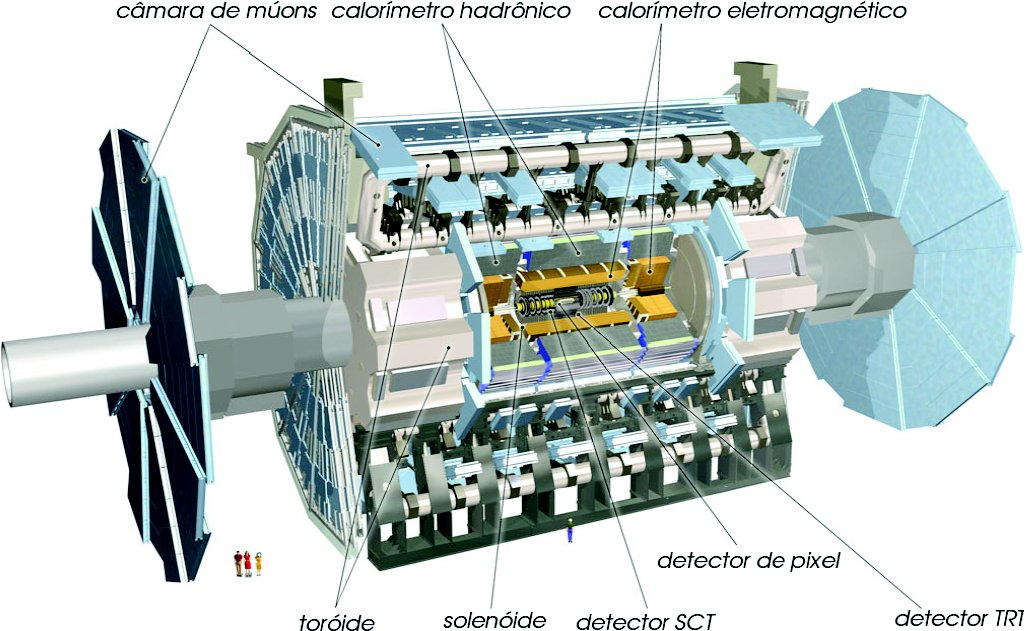
\includegraphics[width=0.8\textwidth]{images/ATLAS_esquema.png}
    \caption[Diagrama ilustrativo do detector ATLAS.]{Diagrama ilustrativo do
    detector ATLAS (adaptado de~\cite{ref:atlas_www}).}
    \label{fig:atlasschema}
\end{figure}

A Figura~\ref{fig:atlassection} apresenta um esquemático da seção transversal do
detector. Os números denotam os diferentes módulos. São eles:

\begin{figure}[H]
    \centering
    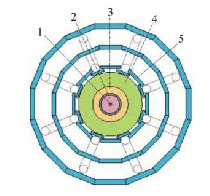
\includegraphics{images/atlas_transversal.png}
    \caption[Seção transversal do detector ATLAS.]{Seção transversal do detector
    ATLAS (extraído de~\cite{ref:TORRES}).}
    \label{fig:atlassection}
\end{figure}


\begin{enumerate}
    \item {\bf Tubo do Feixe:} localizado no centro do detector, aonde passam os
    feixes de prótons.
    \item {\bf Detector de Traços:} composto por uma infinidade de sensores
    altamente segmentados feitos de silício, determina com muita precisão a
    trajetória de partículas carregadas. Estas trajetórias tem natureza curva devido
    ao campo magnético presente no ATLAS. É possível dessa forma estimar o
    momento e a carga da partícula passante.
    \item {\bf Calorímetro Eletromagnético:} determina a energia e o perfil de
    deposição de energia de partículas eletromagnéticas. Está dividido em quatro
    camadas, cada uma com granularidade distinta.
    \item {\bf Calorímetro Hadrônico:} determina a energia e o perfil de
    deposição de energia de partículas hadrônicas, como por exemplo os prótons.
    Está dividido em 3 camadas  com granularidades distintas.
    \item {\bf Espectrômetro de múons:} Os múons são cerca de 200 vezes mais
    pesados do que elétrons. Por essa razão, estas partículas dissipam pouca
    energia ao cruzar o campo elétrico de átomos que estejam no seu caminho.
    Ou seja, tais partículas não são absorvidas por qualquer camada do
    detector.
    O Espectrômetro é composto pela câmaras de múon~\cite{ref:atlas2009}, onde
    um campo magnético é utilizado para curvar a trajetória dos múons. Este
    procedimento aliado a um poderoso sistema de detecção de traço específico,
    permite a medição do momento da partícula.

\end{enumerate}

O Calorímetro Hadrônico e o Espectrômetro de múons serão descritos
detalhadamente ao longo desse capítulo.

\subsection[Sistema de Coordenadas]{Sistema de Coordenadas do ATLAS}

O sistema de coordenadas do ATLAS é um sistema cartesiano que segue a regra da
mão direita. Nesse sistema, apresentado na Figura~\ref{fig:coordinates},
encontram-se~\cite{EGEDE1998}:


\begin{itemize}
    \item o eixo $x$, com lado positivo apontado para o centro da
    circunferência do anel do LHC,
    \item o eixo $z$, seguindo a direção do feixe de partículas, e
    \item o eixo $y$, apontando para cima.
\end{itemize}

\begin{figure}[htpb!]
    \centering
    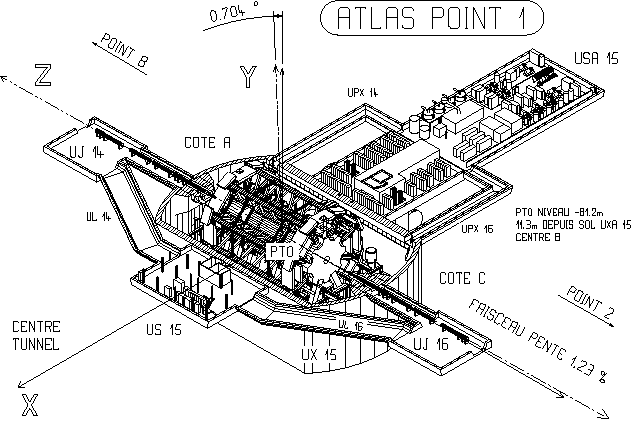
\includegraphics[width=\textwidth]{images/atlas_coordinate_system.png}
    \caption[Sistema de coordenadas do ATLAS]{Sistema de coordenadas do ATLAS (extraído
    de~\cite{EGEDE1998}).}
    \label{fig:coordinates}
\end{figure}

Ao analisar colisões, o sistema cartesiano, mostra-se ineficiente. Nestes
casos, é comum utilizar um sistema que acompanha a direção das partículas
provenientes do ponto de colisão. Assim, são definidas três novas coordenadas
a partir de transformações não-lineares de $x$, $y$ e $z$:

\begin{equation}
    \phi = \arctan\left(\frac{x}{y}\right)
\end{equation}
\begin{equation}
    \Theta = \arctan\left(\frac{x}{z}\right)
\end{equation}
\begin{equation}
    \eta = -\log \left(\arctan\left(\frac{\Theta}{2}\right)\right)
\end{equation}

Ou seja, são adicionadas às coordenadas originais o ângulo azimutal $\phi$ (ao
redor de $z$) e a pseudo-rapidez ($\eta$), que representa a direção da projeção
da partícula, após a colisão.

\subsection{Calorímetro Hadrônico de Telhas}

Calorímetros são fundamentais em detectores hadrônicos de propósitos
gerais~\cite{WIGMANS2000}.  O Calorímetro Hadrônico de
Telhas~\cite{ARIZTIZABAL1994}, conhecido como \emph{TileCal}, desempenha esse
papel.

O sistema de calorimetria do ATLAS é capaz de estimar com grande precisão
medidas de energia e posicionamento de elétrons, prótons, hádrons, taus e jatos.
Também colaboram na identificação e reconstrução de
múons~\cite{AAD2010READINESS}. O TileCal foca na obtenção de medidas precisas de
hádrons, jatos, taus e energia transversa faltante~\cite{MERMOD2008}.

Este calorímetro utiliza cintiladores plásticos como material ativo e ferro
como material que absorve. Compreende a região de pseudo-rapidez $-1,7 < \eta <
1,7$, sendo subdividido em três regiões: uma central  ($-1,0 < \eta < 1,0$),
chamada barril longo~(LB) e dois barris estendidos (EB) localizados nos flancos
do detector ( $0,8 < \|\eta\| < 1,7$), como pode ser visto na
Figura~\ref{fig:tilecalschema}. Ambos, barril longo e estendido, são
segmentados em 64 fatias (módulos) em $\phi$, ou seja, possuem granularidade
$\Delta\phi$ de aproximadamente $0,1$~radianos~\cite{DETECTOR1996TECHNICAL}.

\begin{figure}[htpb!]
    \centering
    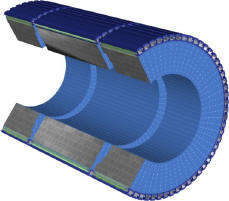
\includegraphics{images/TILECAL_modules_schema.jpg}
    \caption[Diagrama esquemático do TileCal]{Diagrama esquemático do TileCal (extraído
    de~\cite{ref:atlas_www}).}
    \label{fig:tilecalschema}
\end{figure}

Cada módulo é segmentado em três camadas radialmente. Há também a variação
$\Delta\eta$,  igual a $0,1$ nas duas primeiras camadas (denominadas A e BC) e
$0,2$ na terceira camada (denominada D). Deste modo, $\phi$, $\eta$ e a
segmentação radial definem as três dimensões das células do TileCal.  A Figura
~\ref{fig:tilecalgeometry} mostra a distribuição das células dentro de um
módulo.

\begin{figure}[htpb!]
    \centering
    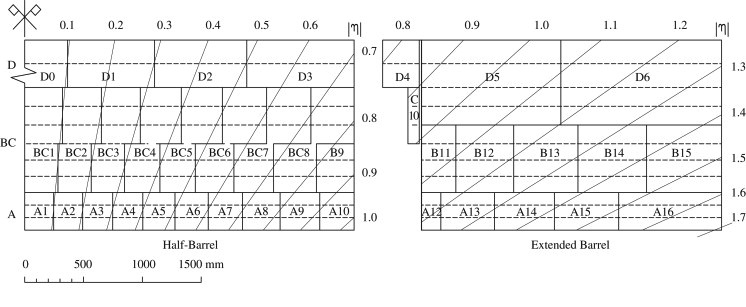
\includegraphics[width=\textwidth]{images/tile_geometry.jpg}
    \caption[Geometria de células do TileCal]{Geometria de células do TileCal.}
    \label{fig:tilecalgeometry}
\end{figure}


Cada célula possui dezenas de placas de ferro e telhas cintilantes. Fibras
óticas deslocadoras de comprimento de onda  (fibras WLS) acopladas às telhas nas
bordas azimutais das células, mostradas na Figura~\ref{fig:tilecalslice},
coletam a luz produzida e a levam até dois tubos fotomultiplicadores
diferentes (PMTs). Cada tubo está conectado a um canal de aquisição, garantindo a
redundância necessária.


A arquitetura de aquisição do TileCal divide o detector em quatro partições. O
barril longo é dividido em duas partições (LBA e LBC) no local entre  plano
perpendicular ao tubo do feixe e o ponto de colisão, e cada barril estendido é
uma partição separada (EBA e EBC)~\cite{AAD2010READINESS}.

A eletrônica de aquisição está localizada em ``gavetas'' inseridas na parte
externa do perímetro do calorímetro. Cada gaveta possui normalmente 45
canais de leitura no barril longo e 32 no barril estendido.

\begin{figure}[htpb!]
    \centering
    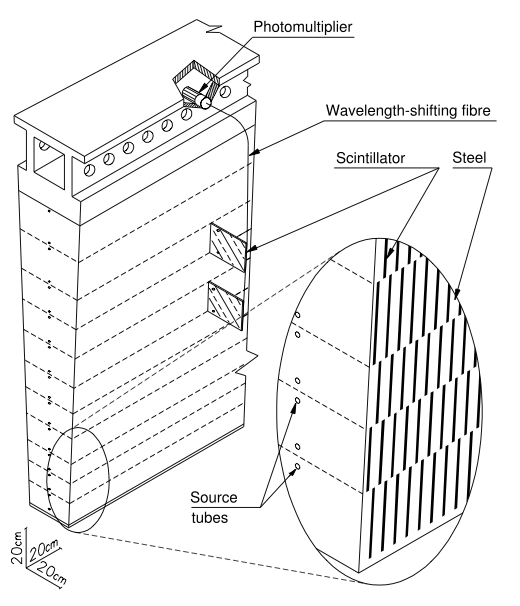
\includegraphics[width=0.5\textwidth]{images/tile_slice.jpg}
    \caption[Estrutura de absorção e amostragem do TileCal]{Estrutura de
    absorção e amostragem do TileCal~(extraído de~\cite{ATLAS2008}).}

    \label{fig:tilecalslice}
\end{figure}

A Tabela~\ref{table:tilefacts} resume a quantidade de canais, de células e de
saídas de trigger para cada tipo de barril.


\begin{table}[htbp!]
  \centering
  \begin{tabular}{ l  r  r  r  }
      \toprule
                         & Canais & Células & saídas de \emph{Trigger}\\
      \midrule
        Barril Longo     & 5760 & 2880 & 1152 \\
        Barril estendido & 4076 & 2302 &  928 \\ [2ex]
        {\bfseries Total}            & 9836 & 5182 & 2080 \\
      \bottomrule
  \end{tabular}
  \caption{Número de canais, células e saídas de Trigger do TileCal.}
  \label{table:tilefacts}
\end{table}

Tanto a eletrônica de \emph{front-end} como as fontes de baixa tensões (LVPS, do
inglês \emph{Low Voltage Power Supplies}) estão localizadas dentro das gavetas e,
portanto, foram projetadas para operar sob condições de elevada radiação e forte
campo magnético~\cite{hruska2007radiation,ARABIDZE2011}.

Os sinais luminosos adquiridos na PMT são transformados em  pulsos elétricos
através de um circuito passivo (\emph{shaper})~\cite{AMES1998}. O pulso é
condicionado para ter uma largura constante, de 50~ns, e amplitude proporcional
à intensidade da quantidade de luz absorvida~\cite{ANDERSON2005}. O pulso
formado é disponibilizado tanto amplificado com um  ganho elevado (HG, do
inglês \emph{high gain}), como também, inalterado (LG, do inglês \emph{low
gain}). A razão nominal entre os dois ganhos é aproximadamente
64:1~\cite{AAD2010READINESS}. O \emph{shaper}, o circuito de amplificação e o
sistema de injeção de cargas para calibração (CIS) estão localizados em um
pequeno circuito impresso conhecido como \emph{3in1 card}~\cite{ANDERSON2005}.

Os sinais HG e LG são amostrados na frequência de 40~MHz utilizando um conversor
analógico digital de 10 bits de faixa dinâmica presente em uma unidade de
gerenciamento de dados~(DMU, \emph{Tile data management unit}). Essa unidade
contêm um \emph{pipeline} de memória que armazena o sinal amostrado por até
6,4~$\mu$s. 

Posteriormente, as amostras são enviadas via cabos de fibra ótica para a
eletrônica de \emph{backend}, localizada fora da caverna principal do
experimento ATLAS. A eletrônica de \emph{backend} determina o período e a
energia do canal das amostras digitalizadas.

A placa \emph{3in1} ainda possui um circuito integrador projetado para medir a
corrente numa determinada PMT durante sessões de calibração com Césio
137~\cite{ANDERSON2009} e interações próton-próton em eventos de \emph{minimum
bias} ocorridos no LHC~\cite{AAD2010READINESS}. O período de integração é de
aproximadamente $14~ms$ e um conversor de 12 bits é utilizado para leitura. A
Figura~\ref{fig:3in1} apresenta o esquemático da placa \emph{3in1} onde todos
seus subsistemas podem ser observados.

\begin{figure}[htpb!]
    \centering
    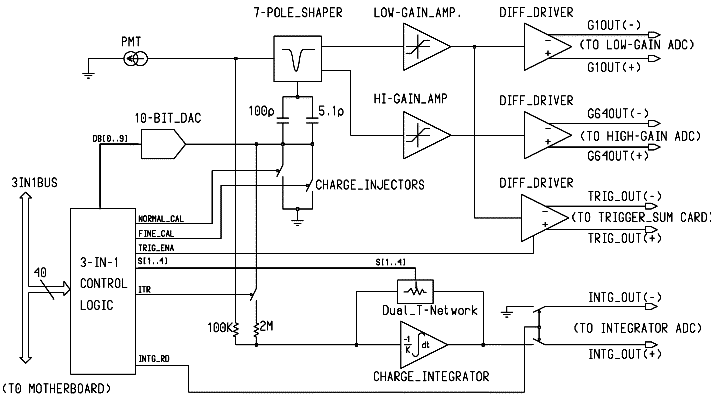
\includegraphics[width=\textwidth]{images/3in1.png}
    \caption[Diagrama de blocos da placa \emph{3in1}]{Diagrama de blocos da
    placa \emph{3in1}(extraído
    de~\cite{ANDERSON2005}).}
    \label{fig:3in1}
\end{figure}

Existem circuitos somadores distribuídos ao longo de uma gaveta e estes são
responsáveis pela interface entre o TileCal e o primeiro nível do sistema de
filtragem do ATLAS~\cite{CERQUEIRA2007}. Cada somador recebe os sinais
analógicos disponibilizados por até 6 placas \emph{3in1}, o que  corresponde a
células localizadas no mesmo intervalo de $\eta$. O sinal de \emph{trigger},
que corresponde a uma ``torre'' de células com  $\Delta\eta \times \Delta\phi =
0,1 \times 0,1$, é formado pela soma analógica dos sinais de entrada. Ele é
posteriormente transmitido junto com  sinais provenientes dos demais
calorímetros do ATLAS para a área externa da caverna do experimento, através de
longos cabos.

Além do sinal da torre, o circuito somador também fornece uma leitura
amplificada da leitura de LG das PMTs localizadas nas células da camada D. Esta
saída é conhecida como ``sinal de múon''. Este sinal é amplificado com um
ganho igual a 255 em relação ao sinal de LG. É um sinal unipolar diferencial,
com excursão máxima de 4Vpp~\cite{CERQUEIRA2007}.

Vale notar que as células da camada D possuem baixa atividade
hadrônica~\cite{CIODARO2009} e, por isso, entende-se que as informações
adquiridas nela  possam ser utilizadas para mitigar o ruído de fundo na
aquisição de múons. Foi esta possibilidade que motivou o presente trabalho de
pesquisa.



\subsection{Sistema de Múons}

O Espectrômetro de Múon ~(MS) compõe a parte externa do ATLAS. Foi projetado
para detectar partículas carregadas que passem pela seção dos calorímetros e
para medir o momento delas na pseudo-rapidez $\|\eta\| < 2,7$~\cite{ATLAS2008}.
Seus principais objetivos para operação são ~\cite{Aad:1275998}:

\begin{itemize}
    \item prover uma medida independente do momento de múons com uma incerteza
    estimada no momento transverso ($p_T$) variando de 3\% em 100~GeV até cerca
    de 10\% em 1~TeV; e 
    \item detectar múons com momentos transversos desde alguns poucos GeV
    (\mbox{$p_T > 3$~GeV}, devido a perda de energia nos
    calorímetros~\cite{ATLAS2008}).
\end{itemize}

O momento de um  múon é determinado a partir da medição de sua trajetória
curvilínea ao passar pelo campo magnético toroidal. Esta trajetória é sempre
perpendicular em relação a principal componente do campo magnético,  o que faz
o cálculo do momento transverso ser independente de $\eta$. O campo magnético é
gerado por três toroides, um na região do barril ($\|\eta\| < 1,1$) e dois nas
regiões dos ``\emph{end-caps}'' ($1,1 < \|\eta\| < 2,7$) com campo total entre 2
e 8~Tm~\cite{Aad:1275998}.

A curvatura do múon é calculada por meio de três estações com câmaras
localizadas ao longo de sua trajetória. Cada estação possui uma acurácia de
$50~\mu$m~\cite{MUONTDR1997}. A Figura~\ref{fig:muonspec} apresenta uma
visualização esquemática do espectrômetro.



\begin{figure}[htpb!]
    \centering
    \begin{subfigure}[b]{\textwidth}
        \centering
        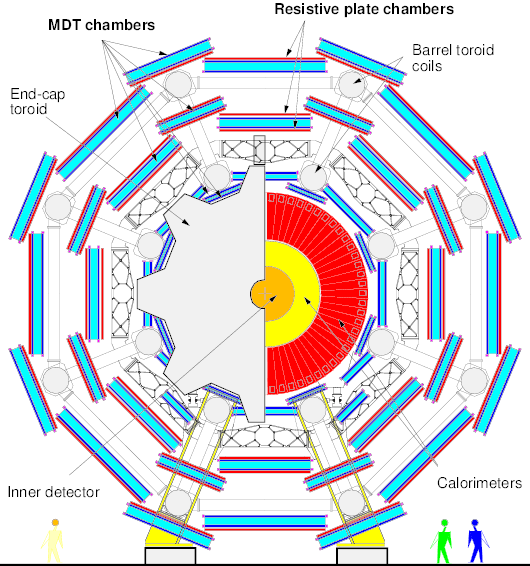
\includegraphics[width=0.9\textwidth]{images/ATLAS-muon-xy-tdr.png}
        \caption{Projeção x-y.}
        \label{fig:muonspecxy}
    \end{subfigure}
    \begin{subfigure}[b]{\textwidth}
        \centering
        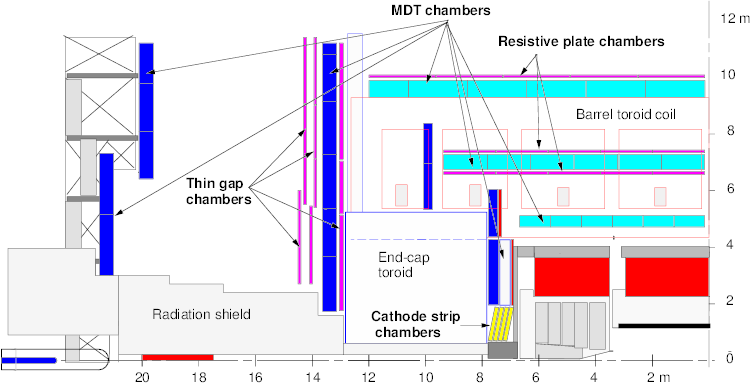
\includegraphics[width=0.9\textwidth]{images/ATLAS-muon-rz-tdr.png}
        \caption{Projeção y-z.}
        \label{fig:muonspecyz}
    \end{subfigure}~\\%
    \caption[Visualização gráfica do Espectrômetro de múons.]{Esquemático do
    espectrômetro de múon. Extraído de~\cite{MUONTDR1997}}
    \label{fig:muonspec}
\end{figure}

As câmaras são divididas em quatro tecnologias: \emph{Cathode Strp Chambers}
(CSC), \emph{Monitored Drift Tubes} (MDT), \emph{Resistive Plate Chambers}
(RPC) e \emph{Thin Gap Chambers} (TGC). O RPC e o TGC são utilizados como
detectores de múons no primeiro nível de filtragem do ATLAS. Já o MDT e CSC são
utilizados para uma medida com alta resolução, porém suas informações só são
utilizadas em eventos pré-selecionados. Como o MDT e o RPC encontram-se na
parte do barril, são de maior interesse para esse trabalho.


\subsubsection*{\emph{Monitored Drift Tubes} (MDT)}

Como já explicado, as câmaras  MDT são responsáveis  pelas medições das
trajetórias curvilíneas de múons. Elas ocupam uma área de $5.500~\text{m}^2$ na região de
rapidez $\|\eta\|<2,7$.

O elemento básico de detecção é um tubo cilíndrico de alumínio com 30~mm de
diâmetro. Em seu interior há um fio de tungstênio-rênio com 50~$\mu$m de
diâmetro, concêntrico com uma acurácia de $10~\mu$m, mantido a 3.080~V. O tubo é
preenchido com um gás não-inflamável composto por argônio~(93\%) e gás
carbônico~(7\%)~\cite{RIEGLER2000}. Os elétrons ionizados pela passagem de uma
partícula carregada são coletados pelo fio condutor, gerando pulsos de corrente
elétrica. Os elétrons que chegam mais rápido ao centro do tubo são exatamente os
que se localizam, no início do processo, no ponto onde a distância entre a
trajetória da partícula e do fio é mínima. Uma série de outros elétrons se
aproximam do fio, gerando picos de corrente por um determinado tempo. Contudo,
apenas o primeiro pico é considerado. A Figura~\ref{fig:mdttube} explica esse
processo: as linhas pontilhadas exemplificam o caminho percorrido por diversos
elétrons, enquanto a linha contínua indica a passagem de um múon.  O gráfico
ilustra que o primeiro pico corresponde ao ponto mais próximo em que partícula
passou em relação ao centro do tubo. Como pode-se supor, a eletrônica de
aquisição e o sistema de alimentação encontram-se nas extremidades do fio, em
oposição entre si~\cite{ATLAS2008}.


\begin{figure}[htpb!]
    \centering
        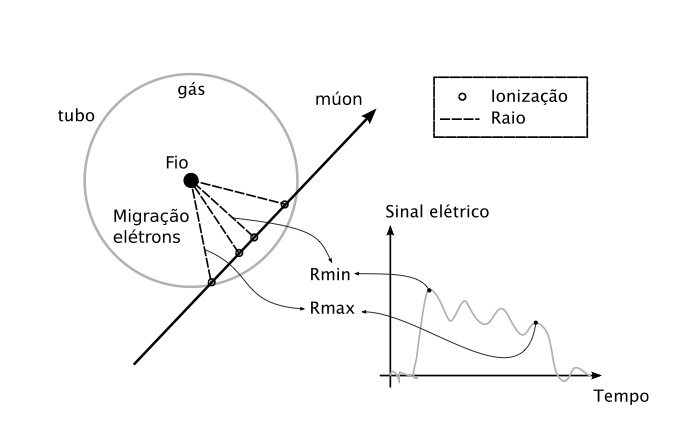
\includegraphics{images/mdt_ion.png}
        \caption[Funcionamento de um tubo do MDT para estimar de maneira precisa a
        trajetória de um múon.]{ Funcionamento de um tubo
        do MDT para estimar de maneira precisa a trajetória de um múon~(adaptado
        de~\cite{MUONTDR1997}).}
        \label{fig:mdttube}
\end{figure}



As câmaras de MDT são montadas a partir de seis camadas de tubos dispostos em um
chassi, três camadas de cada lado, como pode ser visto na
Figura~\ref{fig:mdtchamber}. Os tubos são alinhados de tal maneira que a
espessura do material \emph{multilayer} é em torno de 88~mm. Deste modo, cada
câmara registra seis coordenadas para a trajetória de cada partícula. Na
Figura~\ref{fig:muonspecxy} é possível observar o posicionamento das câmaras em
torno do eixo z.

\begin{figure}[htpb!]
    \centering
        \includegraphics[width=0.8\textwidth]{images/MDTChamber.png}
        \caption[Esquemático de uma câmara MDT.]{Esquemático de uma câmara
        MDT~(retirado de~\cite{MUONTDR1997}).}
        \label{fig:mdtchamber}
\end{figure}


\subsubsection*{\emph{Resistive Plate Chambers} (RPC)}

As câmaras de MDT são relativamente lentas para serem usadas pelo primeiro nível
de filtragem do ATLAS. Por isso, na parte central do barril também encontram-se
as câmaras RPC. Elas estimam o $p_T$ com baixa resolução, porém com rápida
resposta, o que preenche os requisitos do sistema de
filtragem~\cite{MUONTDR1997}. A Figura~\ref{fig:rpclocation} mostra uma seção do
detector e a localização dos RPC (coloridos) em relação aos MDTs. 

\begin{figure}[htpb!]
    \centering
        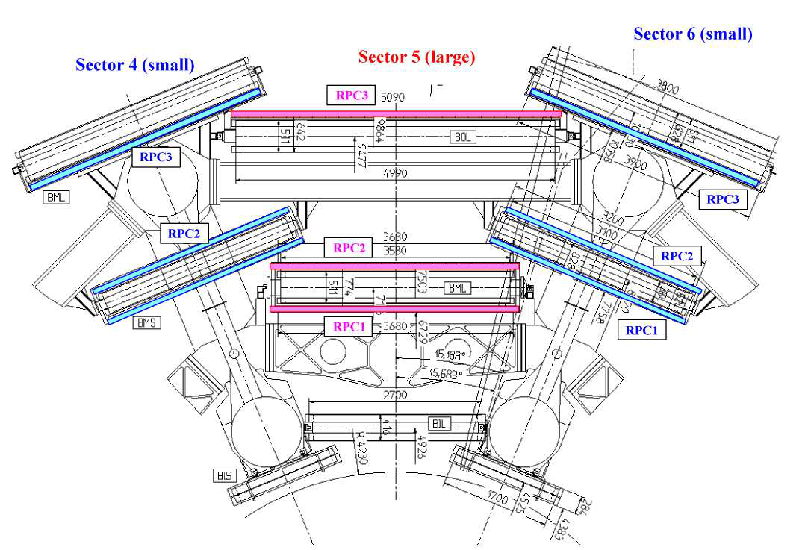
\includegraphics[width=\textwidth]{images/rpc_location.png}
        \caption[Localização dos RPCs na Seção transversal da parte superior do
        barril longo.]{Seção transversal da parte superior do barril longo com
        os RPCs destacados. Na camada do meio encontram-se os RPC1 e RPC2 (ou
        \emph{pivot}), localizados acima e abaixo de um MDT específico. Já o RPC3
        localiza-se acima de um MDT na seção grande e abaixo na outra~(retirado
        de~\cite{Aad:1275998}). As dimensões estão em mm.}
        \label{fig:rpclocation}
\end{figure}

A grande alavanca entre o RPC interno e
externo permite o ~\emph{trigger} selecionar partículas mais energéticas
(10-35~GeV), enquanto as duas câmaras internas focam na escolha de partículas com
baixo $p_T$ (6-10~GeV). A Tabela~\ref{table:rpc_segmentation} apresenta a
segmentação do sistema RPC através da contagem de câmaras e da distância radial
de cada RPC.

Cada plano do RPC é um conjunto de duas chapas resistivas feitas de baquelite
(resina plástica resistente ao calor). Essas chapas são postas distanciadas uma
da outra por 2~mm. O espaço é preenchido por um gás ionizado. O campo
elétrico aplicado entre as duas placas é igual $ 4,9~kV/mm$~\cite{ATLAS2008}.
Fitas metálicas são dispostas ao longo de $\eta$ e $\phi$, fornecendo a
granularidade requerida pelo ATLAS~\cite{MUONTDR1997, POLINI2012}.

As partículas que cruzam o detetor ionizam o gás do RPC. Elétrons são liberados
e atraídos pelo campo elétrico até as extremidades da câmara, onde são coletados
pelas fitas metálicas. Os sinais das fitas são adquiridos por uma eletrônica
simples que compara com padrões previamente determinados~\cite{MUONTDR1997}. A
distribuição espacial e temporal dos pontos sensibilizados pela passagem de um
múon é suficiente para estimar o seu momento transverso~\cite{ANULLI2009}.

\begin{table}[htbp!]\footnotesize
  \centering
  \tabcolsep=0.08cm
  \begin{tabular}{ m{1.5cm}   m{1.5cm}  m{1.5cm}  m{1.5cm}  m{1.5cm} m{1.5cm} m{1.5cm}  m{1.5cm}  m{1.5cm}  }
       \multicolumn{1}{c}{}& \multicolumn{4}{c}{Setor pequeno}& \multicolumn{4}{c}{Setor Grande} \\
        \cmidrule(r){2-5}
        \cmidrule(r){6-9}
      Nome & Unidades & Câmaras & Raio & Distância ao Pivot & Unidades & Câmaras & Raio & Distância ao Pivot \\
      \midrule
      RPC1 & 148 & 84 & 7820  & 545  & 149 & 94 & 6800 & 678 \\
      RPC2 & 148 & 84 & 8365  &      & 149 & 94 & 7478 &     \\
      RPC3 & 176 & 92 & 10229 & 1864 & 192 & 96 & 9832 & 2354\\
      \bottomrule
  \end{tabular}
  \caption{Segmentação do sistema RPC com 544 câmaras e 962 unidades. Todas as
  dimensões estão em mm.}
  \label{table:rpc_segmentation}

\end{table}
\subsubsection*{Geometria}

As três camadas do MS estão distribuídas de acordo com a distância do feixe de
partículas do ATLAS. A Figura~\ref{fig:muonsector} mostra a divisão lógica e a
numeração dada ao MS. Essas camadas são chamadas de \emph{inner}, \emph{middle}
e \emph{outer} localizadas respectivamente a 3,5~m, 5~m e 7~m. O espectrômetro
é dividido azimutalmente em 64 setores (chamados setores de \emph{trigger}),
pequenos ou grandes.

\begin{figure}[htpb!]
    \centering
    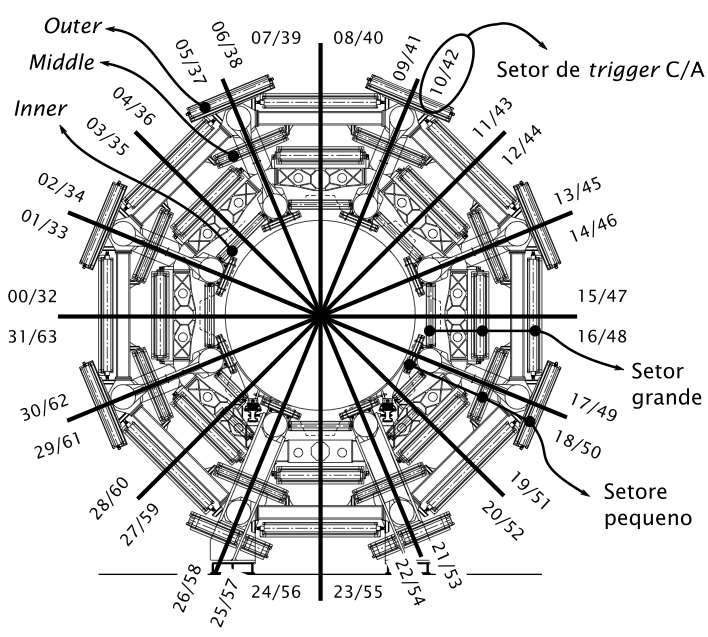
\includegraphics[width=0.8\textwidth]{images/muon_sectors.png}
    \caption{Setores de \emph{trigger} do Espectrômetro de Múons}
        \label{fig:muonsector}
\end{figure}

Cada câmara no plano \emph{pivot} define duas regiões de \emph{trigger} em
$\eta \times \phi$, chamadas PAD~\cite{ANULLI2009}, com granularidade $0,2
\times 0,2$.  Dentro de uma PAD são definidas regiões de interesse (RoI, do
inglês \emph{Regions of Interest}) que ocupam aproximadamente $0,1 \times 0,1$
em $\eta \times \phi$. A Figura~\ref{fig:muonroi} mostra o mapeamento dos RPC
em RoIs. Existem áreas em $\phi$ onde diferentes setores se sobrepõem. Múons
que cruzam essas regiões são registrados por ambas, porém somente uma será
considerada pela eletrônica de aquisição, acabando com a
ambiguidade~\cite{ANULLI2009}.


\begin{figure}[htpb!]
    \centering
    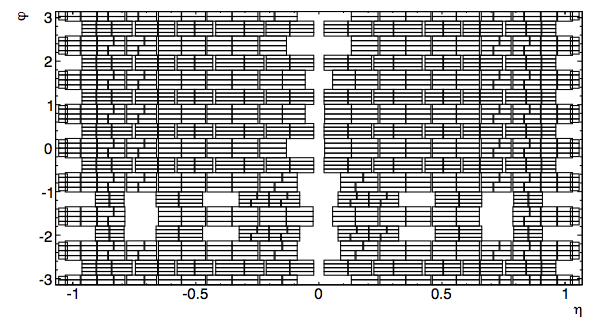
\includegraphics[width=0.8\textwidth]{images/muonroi.png}
    \caption{Mapa de RoIs para o RPC}
        \label{fig:muonroi}
\end{figure}

%%End of chapter
%%%%%%%%%%%%%%%%%%%%%%%%%%%%%%%%%%%%%%%%%%%%%%%%%%%%%%%%%%%%%%%%%%%%%%%%%%

%\subsection{A descoberta do bóson de Higgs}
%\begin{figure}[htpb!]
%    \centering
%    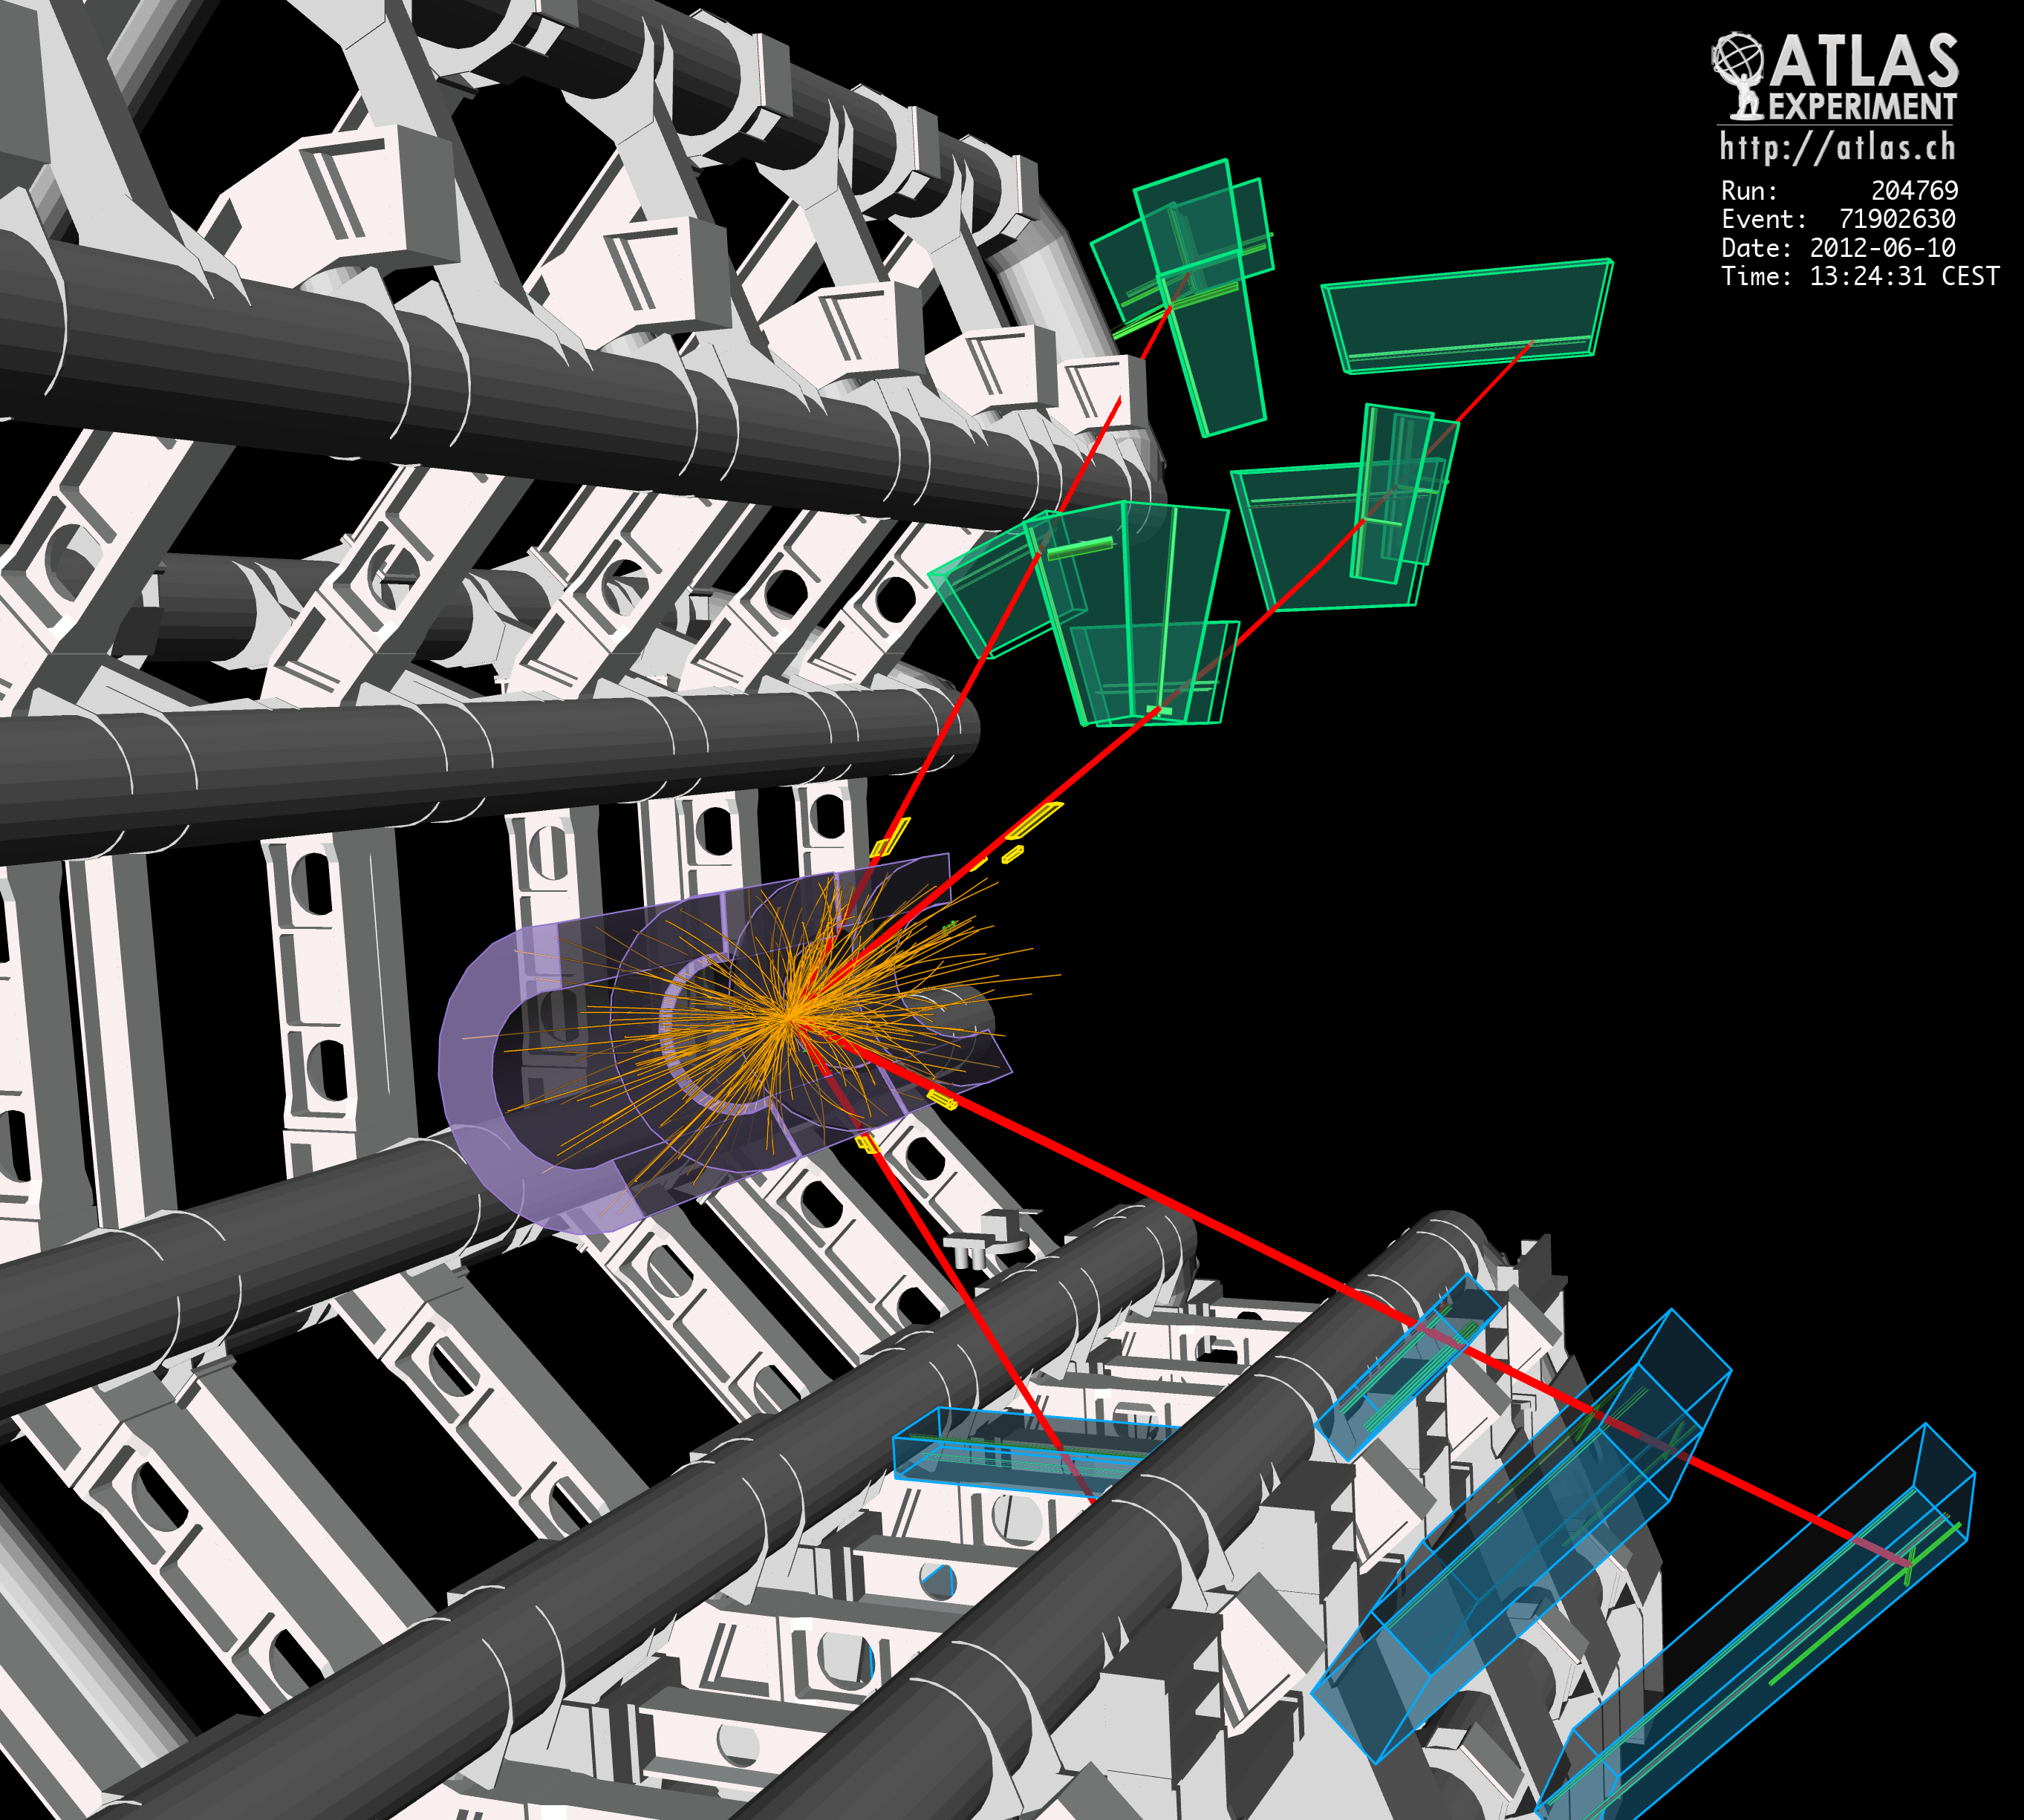
\includegraphics[width=\textwidth]{images/run204769_evt71902630_MSonly_hres.png}
%    \caption{Reprodução de um evento candidato a $H \rightarrow 4\mu$ (extraído
%    de~\cite{ref:atlas_www}).}
%\end{figure}

  %% Chapter Trigger

\chapter{Sistema de Filtragem do ATLAS}

O ATLAS apresenta três níveis de seleção de eventos: Primeiro Nível~(L1),
Segundo Nível~(L2) e o \emph{Event Filter}~(EF). O L2 e o EF juntos são chamados
de \emph{High Level Trigger} (HLT). O L1 é implantado utilizando placas
eletrônicas especialmente projetadas para a tarefa, enquanto o HLT é quase 
totalmente composto por dispositivos de rede e computadores disponíveis
comercialmente~\cite{ref:2010performance}.

O L1 procura por assinaturas de múons com momento elevado, elétrons/prótons e
jatos. Nesta fase, são considerados apenas detectores com granularidade restrita
como, o RPC do múon e os subsistemas dos calorímetros eletromagnético e
hadrônico~\cite{LEVEL1TRIGGER}. A taxa máxima de aquisição projetada para o L1 é
igual a 75~kHz, e pode ser aumentada até 100~kHz após uma atualização do
sistema~\cite{ATLAS2008}. A decisão de rejeitar ou não um evento deve ser tomada
dentro de 2,5~$\mu$s após a tomada de dados.

O L2 é alimentado pelas RoIs. Essas são as regiões do detector ATLAS onde o L1
identificou possíveis objetos de interesse. O L2 usa as coordenadas, a energia e
o tipo de assinatura para limitar a quantidade de dados que será transmitida
dos instrumentos de leitura do detector. Nesse momento, a taxa de eventos cai
para 3,5~kHz, com um processamento médio de aproximadamente
40~ms~\cite{ATLAS2008}.

O EF usa análise \emph{offline} de eventos já reconstruídos para reduzir a taxa
de armazenagem para cerca de 200~Hz. Os eventos selecionados e gravados serão
utilizados em análises subsequentes~\cite{ARMSTRONG2004}. A
Figura~\ref{fig:triggersystem} representa graficamente o fluxo de informações do
sistema de filtragem.

\begin{figure}[htpb!]
    \centering
    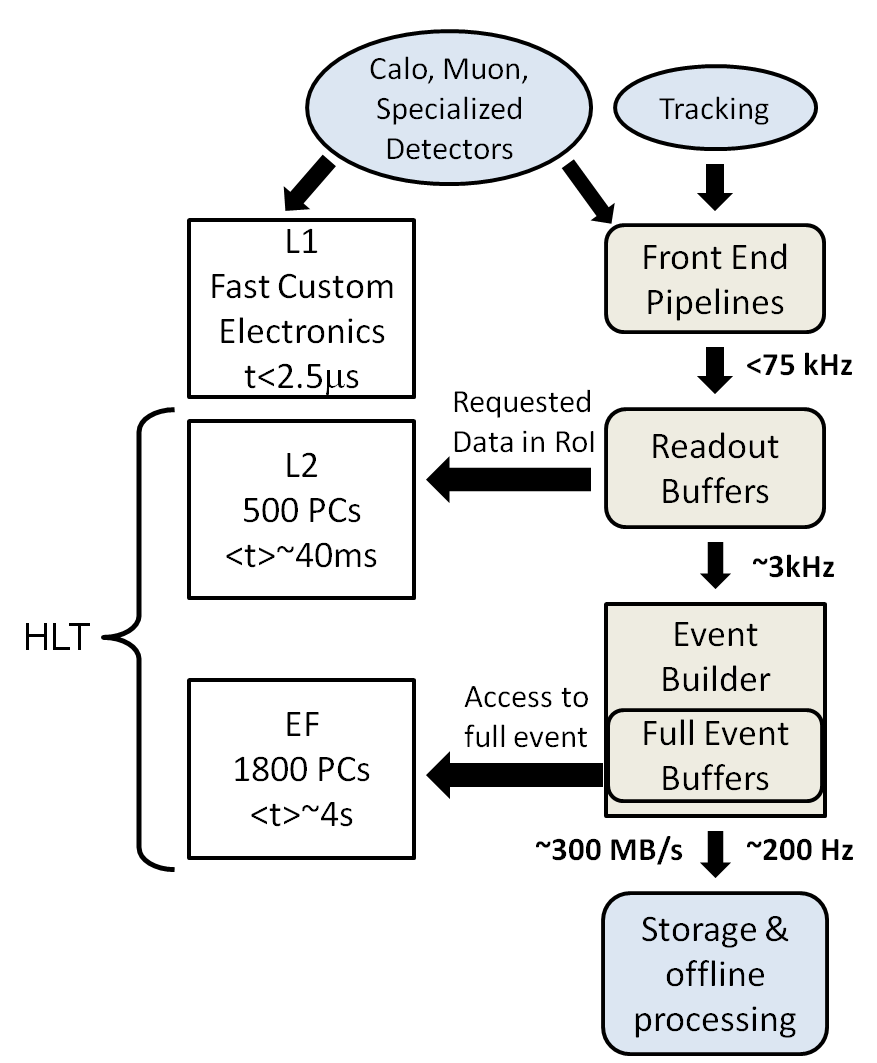
\includegraphics[width=8cm]{images/atlas_trigger_system.png}
    \caption[Esquemático do sistema de filtragem do ATLAS.]{Esquemático do
    sistema de filtragem do ATLAS. Extraído de~\cite{ref:2010performance}.}
    \label{fig:triggersystem}
\end{figure}

Os algoritmos utilizados no HLT usam a granularidade e precisão máxima para os
dados dos calorímetros e câmaras de múon, além de dados provenientes do
detector de traços para refinar a seleção~\cite{ATLAS2008}. Quanto mais
informações sobre a energia depositada, melhor a determinação de limiares de
corte. Já a reconstrução da trajetória na parte mais interna do detector
permite a diferenciação de partículas, como, por exemplo, elétrons e prótons.

O sistema de aquisição de dados (DAQ, do inglês \emph{Data AcQuisition} ) recebe
os eventos, na mesma taxa do que no L1, e retêm-os em um \emph{buffer}.
Posteriormente, os dados são transmitidos através de uma comunicação
ponto-a-ponto~\cite{ATLAS2008}.  Qualquer informação requerida pelo L2 é
transmitida, geralmente relacionadas às RoIs. Os eventos que passarem por todos
os critérios de seleção do L2 serão compilados (o chamado \emph{event-building})
e passados pelo DAQ para o EF~\cite{ATLAS2008}. Finalmente, os eventos
selecionados serão armazenados permanentemente~\cite{VAN2009}.

Para controlar todo tráfego de dados durante a cadeia de seleção, o DAQ ainda
fornece a configuração, controle e monitoramento do detector ATLAS durante a
tomada de dados~\cite{ATLAS2008,MIOTTO2010}.

O sistema de controle do detector (DCS,  do inglês \emph{Detector Control
System}) é o responsável pela supervisão e operação do \emph{hardware} (sistema
de gás, fontes de alimentação, sistema de refrigeração, etc.)~\cite{PPOY2008}.

\section{Primeiro Nível de Filtragem}

O fluxo de dados do L1 é mostrado na Figura~\ref{fig:l1schema}. Nesse nível, a
seleção inicial é realizada baseada na informação dos calorímetros e do
espectrômetro de múon.

\begin{figure}[htpb!]
    \centering
    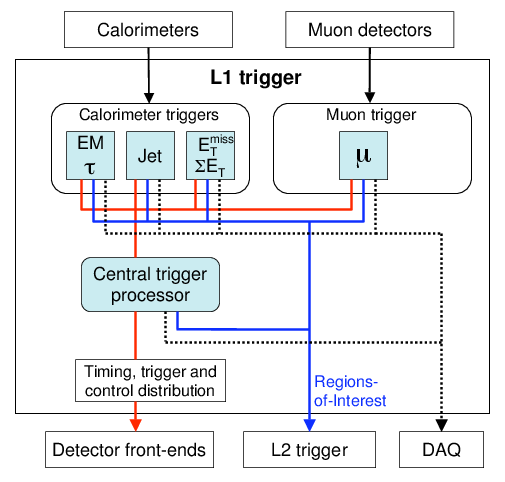
\includegraphics[width=8cm]{images/l1-schema.png}
    \caption[Diagrama de blocos do L1.]{Diagrama de blocos do L1. As decisões do L1 são tomadas no
    CTP~(Processador de Filtragem Central), tomando em conta os resultados dos
    sistemas de calorimetria e de múons. O fluxo para a eletrônica de
    \emph{front-end}, para o L2 e para o DAQ, são mostradas em vermelho, azul e
    preto, respectivamente. Retirado de ~\cite{ATLAS2008}.}
    \label{fig:l1schema}
\end{figure}

O L1 de calorimetria (L1Calo) tem como principal objetivo na identificação de
partículas como elétrons, fótons, jatos e o $\tau$-léptons\footnote{O
$\tau$-lépton, ou simplesmente tau, é uma partícula elementar similar ao
elétron, com carga elétrica negativa e spin de
$\frac{1}{2}$~\cite{ATLAS2011TAU}.} que decaiam em hádrons. Eventos com grande
energia transversa também são almejados. 

O L1 do sistema de múon baseia-se nos sinais das câmaras de trigger: RPCs na
região do barril e TGC's no \emph{end-caps}. A seleção ocorre através de
padrões consistentes com múons com alto momento transverso originados na região
de interação. Sua lógica disponibiliza 6 limiares para $p_T$
independentes~\cite{ATLAS2008}. A informação que o L1 disponibiliza é a
quantidade de múons que atingiram cada limiar. É importante ressaltar que nunca
um múon é contado em dois limiares diferentes~\cite{ATLAS2008}.


As decisões tomadas pelo L1 são feitas no Processador de  Filtragem
Central~(CTP, do inglês \emph{Central Trigger Processor}), que combina as
informações de todos os tipos de objetos.  Dependendo das características
extraídas, o evento é classificado em até 256 itens separados. A
Tabela~\ref{table:l1objects} apresenta um resumo dos objetos disponíveis para
L1, os limiares de seleção e suas respectivas frequências obtidas em 2012.

\begin{table}[htbp!]\footnotesize
  \centering
  \tabcolsep=0.08cm
  \begin{tabular}{ l  m{5cm} c c }
      \toprule
                                          & Objeto de interesse & Limiar de seleção (GeV) & Frequência~(kHz) \\
      \midrule
      \multirow{2}{*}{Léptons simples}    & Múon $p_T > 25$~GeV        &      15             & 8        \\
                                          & Elétron $p_T > 25$~GeV     &      18             & 17       \\
      \midrule
      \multirow{4}{*}{Léptons duplos}     & 2 Múons $p_T > 15$~GeV     &      2x10           & 1        \\
                                          & 2 Múons $p_T > 20,10$~GeV  &      15             & 8        \\
                                          & 2 Elétrons $p_T > 15$~GeV  &      2x10           & 6        \\
                                          & 2 Taus $p_T > 45$~GeV      &      15, 11         & 12       \\
      \midrule
      \multirow{2}{*}{Fótons  duplos}     & 2 Fótons $p_T > 25$~GeV    &   2x10              & 6        \\
                                          & 2 Fótons \emph{loose} $p_T > 40,30$~GeV & 12, 16 & 6        \\
      \midrule
      Outros                              &                            &                     & $\sim 6$ \\
      \midrule
      {\bf Total}                         &                            &                     & $\sim 75$ \\
      \bottomrule
  \end{tabular}
  \caption[Taxa de eventos para os objetos de interesse no L1.]{Taxa de eventos
  para os objetos de interesse no L1. Retirado de~\cite{PETERSEN}.}
  \label{table:l1objects}
\end{table}

Neste ponto, apenas o número de ocorrências de objetos selecionados é levado em
consideração (ou \emph{flags} indicando quais limiares foram alcançados). As
informações sobre a localização geométrica de um objeto é retida nos
processadores de \emph{trigger} dos sistemas de calorimetria e de múons. Assim
que o evento for aceito no L1, essas informações serão mandadas como RoIs para o
L2, onde serão usadas no processo de seleção.

Uma função fundamental do L1 é identificar o \emph{bunch-crossing} de interesse.
O \emph{bunch-crossing}, ou simplesmente BC, é o termo atribuído à injeção de
pacotes de prótons no acelerador ocorrida a cada 25~ns. Este curto espaço de
tempo torna a tarefa um desafio. No caso do \emph{trigger} do múon, o tamanho do
detector implica em um tempo de percurso maior que o intervalo entre as injeções
de pacote. Já os sinais de calorimetria duram tipicamente quatro vezes mais que
o \emph{bunch-crossing}~\cite{ATLAS2008}.

Enquanto a decisão do \emph{trigger} é realizada, as informações de todos os
canais do ATLAS estão armazenadas em memória. Essas memórias estão localizadas
na eletrônica de \emph{front-end} e frequentemente está submetida a altos
níveis de radiação, onde o acesso é muito difícil~\cite{ATLAS2008}. É desejável
que o \emph{pipeline} de memória seja o menor possível. O projeto da eletrônica
de \emph{front-end} requer que essa latência seja de no máximo 2,5~$\mu$s.
Cerca de 1~$\mu$s desse tempo é deixado para propagação dos dados no
cabeamento.

\subsection*{Primeiro Nível de Filtragem da Calorimetria}

As 7.000 saídas analógicas dos calorímetros eletromagnético e hadrônico são
tratadas pelo \emph{L1Calo}. A Figura~\ref{fig:L1CALO} apresenta sua
arquitetura. Este é um sistema digital localizado na parte externa do ATLAS
constituído por 3 subsistemas:

\begin{figure}[htpb!]
    \centering
    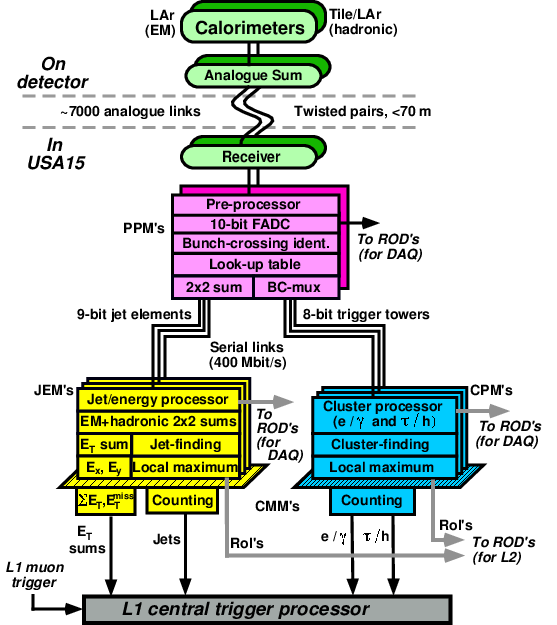
\includegraphics[width=12cm]{images/CaloTrigArch.png}
    \caption[Esquemático do funcionamento do \emph{L1Calo}.]{Esquemático da
    arquitetura do \emph{L1Calo}~(Extraído de~\cite{ATLAS2008}).}
    \label{fig:L1CALO}
\end{figure}


\begin{description}
    \item[Módulo de pré-processamento] Responsável por digitalizar os sinais
    analógicos recebidos e utiliza um filtro que os associa com o
    \emph{bunch-crossing} específico. Utiliza  ainda uma tabela de
    referência para fornecer os valores de energia transversa que serão usados
    nos algoritmos subsequentes.
    \item[Processadores de \emph{clusters}~(CP)] Responsável por identificar
    candidatos a elétrons/prótons e $\tau$-léptons através de limiares
    relacionados a deposição de energia.
    \item[Processadores de Jatos e Energia~(JEM)] Recebe elementos de interesse
    e os usa para identificar jatos e calcular a energia transversa total.
\end{description}

 A descrição completa de cada um dos blocos e da eletrônica responsável por essa
 etapa da filtragem de eventos pode ser encontrada em~\cite{ACHENBACH2008}.



\section{Sistema de Filtragem de Alto Nível}

O sistema de filtragem de alto nível do ATLAS (\emph{High Level Trigger} - HLT)
é composto pelo L2  e EF, ambos implementados em \emph{software} com linguagem
de programação de alto nível. A Figura~\ref{fig:tdaq_diagram} apresenta os
detalhes desta parte do sistema de filtragem. O HLT
está dividido em duas partes: a aquisição e controle de dados e o
processamento dos eventos produzidos pelo ATLAS. Estas duas partes, juntas, são
referidas como TDAQ (\emph{Trigger and Data Aquisition})~\cite{NEGRI2012,ref:TORRES}.

\begin{figure}[hbtp!]
\centering
    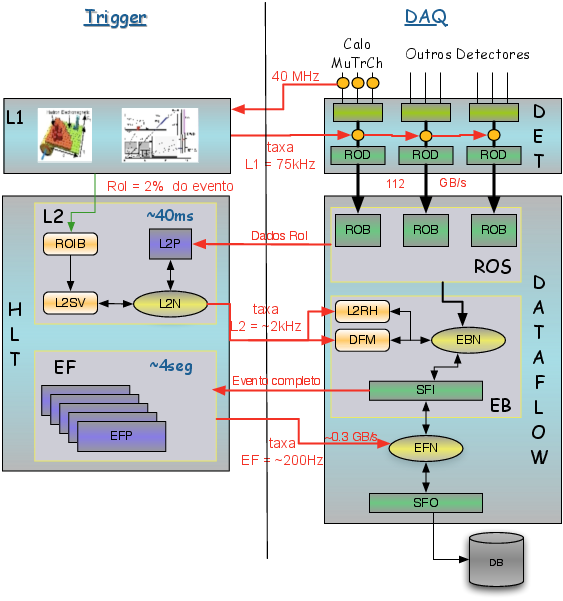
\includegraphics[height = 10cm]{images/tdaq_diagram.png}
    \caption[Diagrama em blocos do sistema de filtragem de alto nível.]{Diagrama
    em blocos do sistema de filtragem de alto nível (Retirado
    de~\cite{TORRES2009}).}
    \label{fig:tdaq_diagram}
\end{figure}


Após a filtragem do L1, os eventos aprovados ficam disponíveis na forma de
fragmentos nos sistemas de leitura (\emph{Read-Out Systems - ROS}).  Além
disso, a informação a respeito das RoIs etiquetadas pelo L1 é enviada para o
construtor de RoI (\emph{RoI Builder} - RoIB). Este agrupa os fragmentos de
informação gerados pelos diferentes detectores do ATLAS e transmite o registro
gerado por este agrupamento para um supervisor do segundo nível (\emph{L2
Supervisor - L2SV}), que ficará responsável por atribuir a RoI recebida a uma
unidade de processamento do segundo nível  (\emph{L2 Processing Unit} - L2PU).
A L2PU então valida a etiqueta do L1, usando a plena granularidade dos
detectores, e retorna o resultado para o L2SV. Este envia o resultado para o
gerenciador de fluxo de dados (\emph{Dataflow Manager - DFM}), para que o
evento seja apagado em caso de rejeição, ou propagado para o filtro de eventos,
caso seja aprovado.  O DFM seleciona um dos processadores SFI (\emph{Sub-Farm
Input}) para que o mesmo solicite aos ROS toda a informação disponível do
evento em questão. Uma vez a informação disponível, o SFI seleciona um dos
processadores do filtro de eventos (\emph{EF Processor - EFP}), para que o
mesmo realize análises detalhadas, usando toda a informação disponível para
cada evento, gerando, assim, a decisão final do sistema de filtragem. Os
eventos finalmente aprovados são enviados aos processadores SFO (\emph{Sub-Farm
Output}) para que possam ser armazenados em mídia permanente, permitindo
posterior análise \emph{offline}~\cite{RIU2008}.

Todo o segundo nível de filtragem foi desenvolvido utilizando, o máximo
possível, tecnologias padronizadas (comerciais)~\cite{ANJOS2004}, visando
fácil reposição de material e implementação simplificada. Todos os
processadores são de uso geral (tipo PC) e praticamente todas as comunicações
entre estes dispositivos são feitas através de \emph{switchs} Gigabit Ethernet,
devido à velocidade, confiabilidade e padronização do protocolo. Todas as
aplicações também estão desenvolvidas utilizando técnicas de orientação a
objetos e implementadas em C++~\cite{SCHILDT2003}.


\section{Seleção de Múons}

Múons detectados pelo RPC, no L1, alimentam os algoritmos do HLT (High-Level
Trigger). Além de utilizar informação com granularidade fina, estes algoritmos
tem acesso à informação de trajetória do ID (\emph{Inner Detector}) e da energia
perdida pelo múon nos calorímetros. Com isso, não só o momento transverso do
múon pode ser refinado, mas também informações sobre a origem física desse múon.
Essas informações são necessárias para a identificação dos processos físicos que
aconteceram no detector.

\subsection{Seleção no L1}

O primeiro nível de filtragem para múons, conhecido como \emph{L1Muon}, busca
pela combinação de cruzamentos entre partículas e as diferentes câmaras do
espectrômetro, afim de identificar múons em 6 patamares de momento
transverso~($p_T$) distintos.

Ao detectar o cruzamento de um múon na primeira estação, o sistema projeta
janelas de visualização nas outras camadas. Estas janelas foram pré-calculadas
usando simulações de Monte Carlo. Cada combinação de pontos de cruzamento indica
o $p_T$ da partícula~\cite{BUTTINGER2012}. Aproximadamente 15~kHz dos 75~kHz da
banda de seleção do nível 1 de filtragem são reservados para eventos de múons. A
Figura~\ref{fig:MSMUON} mostra dois exemplos de múons passando pelo
espectrômetro. Nela está representada uma seção transversal do detector ATLAS e
a representação de duas janelas de visualização projetadas pelo sistema de
filtragem: uma para um múon de baixo $p_T$ e outra para o de alto $p_T$.


\begin{figure}[htpb!]
    \centering
    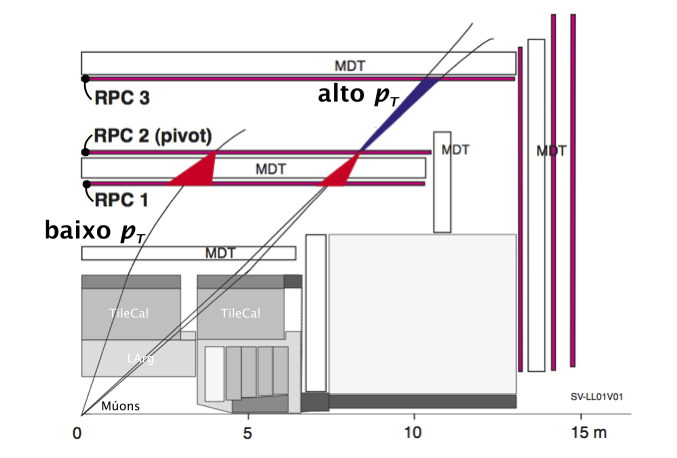
\includegraphics[width=11cm]{images/MS_transversal.png}
    \caption[Seção transversal do detector ATLAS, mostrando exemplos de duas
    partículas cruzando as câmaras do espectrômetro e as respectivas projeções
    do \emph{L1Muon}]{Seção transversal do detector ATLAS, mostrando exemplos de duas
    partículas cruzando as câmaras do espectrômetro e as respectivas projeções
    do \emph{L1Muon} (Adaptado de~\cite{BUTTINGER2012}).}
    \label{fig:MSMUON}
\end{figure}

O \emph{L1MUON} é configurado para encontrar os seguintes patamares de
seleção~\cite{BUTTINGER2012}:

\begin{description}
    \item[MU0] Aceita múons com qualquer valor de $p_T$. Basta a partícula
    cruzar duas estações do mesmo setor do espectrômetro. Esse patamar foi
    substituído pelo MU4 a partir da metade de 2011.
    \item[MU4] Seleciona múons que cruzam duas estações de coincidência do mesmo
    setor com $p_T$ aproximadamente igual a 4~GeV.
    \item[MU6] Seleciona múons com $p_T$ acima de aproximadamente 6~GeV. Requer
    que pelo menos duas estações do RPC sejam atingidas ou as três coincidências
    no TGC.
    \item[MU10] Seleciona múons com $p_T$ acima de aproximadamente 10~GeV. Possui
    as mesmas regras de coincidência do MU6, porém projeta janelas menores.
    \item[MU11] Seleciona múons com $p_T$ acima de aproximadamente 11~GeV. Exige
    três coincidências em todas as regiões (RPC ou TGC) do sistema. Não existe
    resolução suficiente de energia para diferenciar os patamares MU11 e MU10.
    \item[MU15] Seleciona múons com $p_T$ acima de aproximadamente 15~GeV. Exige
    a passagem do múon nas três estações.
    \item[MU20] Seleciona múons com $p_T$ acima de aproximadamente 20~GeV. Possui
    as mesmas regras de coincidência do MU15, porém projeta janelas menores.
\end{description}

Algumas regiões do detector não são cobertas pelo RPC devido a questões
geométricas~\cite{MUONTDR1997}. Nessas regiões, o múon não pode ser classificado
como MU11, MU15 ou MU20, mesmo que o valor de $p_T$ o qualifique para tal
patamar. Adicionalmente, cerca de 1\% das placas RPC pararam de funcionar devido
à problemas no sistema de alimentação~\cite{ATLAS-CONF-2012-099}, aumentando
assim o número de regiões sem cobertura. Nesses casos, os eventos são marcados
como MU10.

A partir de 2011, observou-se um aumento na taxa de múons marcados com MU10.
Isso deve-se a instalação de uma blindagem adicional entre a região dos barris e
os \emph{end-caps}.

\subsection{Seleção no HLT}

A seleção de múons no L2 utiliza informações com granularidade plena para as
RoIs passadas pelo L1, melhorando a estimativa da posição e do momento
transverso atráves de algoritmos otimizados para uma rápida seleção e uma
eficiente rejeição de ruído de fundo~\cite{VENTURA2010}. Ao invés de utilizar a
informação proveniente do RPC, esses algoritmos processam dados adquiridos
pelas câmaras de precisão (MDT no caso da região do barril). Os algoritmos do EF
também tem acesso à resolução pena do detector~\cite{KORDAS2007}.


A Figura~\ref{fig:MUONHLTFLOW} apresenta o fluxo de dados entre os diversos algoritmos de
seleção de múons do L1, L2 e EF. Os tempos totais e banda de frequência são do
experimento ATLAS como um todo.

\begin{figure}[htpb!]
    \centering
    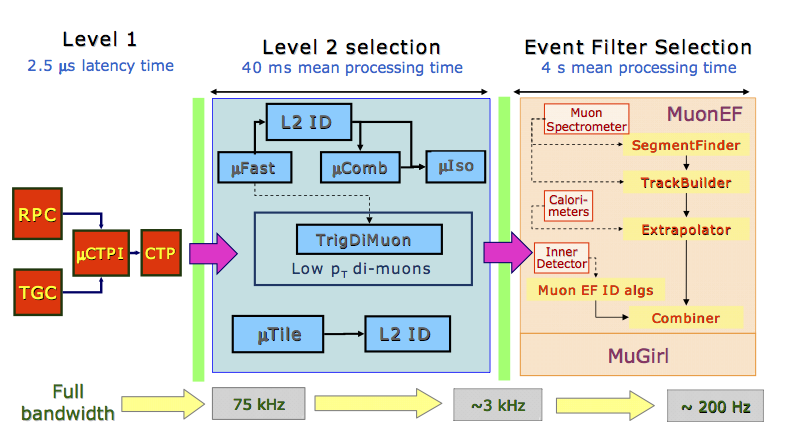
\includegraphics[width=\textwidth]{images/hlt_flow_muon.png}
    \caption[ Fluxo de dados entre os algoritmos do filtro de seleção para múons
    do ATLAS] {Fluxo de dados entre os algoritmos do filtro de seleção para
        múons do ATLAS (Retirado de~\cite{VENTURA2010}).}
    \label{fig:MUONHLTFLOW}
\end{figure}

\subsubsection{Algoritmos do L2 para Selecionar Múons}

O primeiro algoritmo do L2, o \emph{muFast}~\cite{DIMATTIA2003}, visa confirmar
ou descartar candidatos a múons escolhidos no L1. Através dele, são selecionados
tubos do MDT próximos a trajetória projetada pelo L1. Em cada estação, um ajuste
linear é realizado para obter a interseção entre a passagem do múon e a própria
estação, melhorando a reconstrução do trajeto percorrido pela
partícula~\cite{DIMATTIA2011}.

O algoritmo \emph{muComb} combina as informações provenientes do ID com a
trajetória do múon dentro do MS~\cite{VENTURA2010}. Desta maneira, é possível
extrapolar as trajetórias reconstruídas pelo ID até o MS e rejeitar múons
provenientes de decaimentos de píons e káons, assim como falsos alarmes e
raios-cósmicos~\cite{COSMICRAY2010}.


O terceiro algoritmo se baseia na informação extraída pelo \emph{muComb} para
refinar ainda mais a reconstrução do múon. Esse algoritmo, \emph{muIso}, é
utilizado para distinguir um múon isolado e um não isolado. Assim como o
\emph{muComb}, o \emph{muIso} pode ser utilizado para rejeitar múons oriundos de decaimentos
de hádrons. Porém, diferentemente do \emph{muComb}, informação de calorimetria é
utilizada~\cite{VENTURA2010}.


O \emph{muTile} foi implementado para aumentar a eficiência em múons com momento
transverso baixo. Para tal, ele baseia-se na energia depositada na última camada
do TileCal (célula D). Se a energia verificada for compatível com a de um múon,
então as demais células daquela torre são analisadas. Se o valor de todas as
células satisfazer os cortes energéticos do algoritmo, considera-se que a torre
foi cruzada por um múon~\cite{USAI2004}.

\subsubsection{Algoritmos do EF para Selecionar Múons}

Dois algoritmos fazem parte do filtro de eventos de múons: o \emph{TrigMuonEF} e
o \emph{TrigMuGirl}. Ambos são baseados nas ferramentas \emph{offline} de
reconstrução de múons~\cite{ARMSTRONG2004}.
Os algoritmos para deteção de múons do filtro de eventos seguem as mesmas
estratégias dos algoritmos do L2, contudo por possuir maior tempo de latência,
4~s contra 40~ms do L2, pode acessar mais informações e obter resultados mais
apurados. Assim, a principal tarefas deles é confirmar os candidatos de múons
validados pelo L2~\cite{VENTURA2010}.

  \chapter{Identificação de partículas}

Este capítulo descreve a elaboração de um modelo capaz de discriminar partículas
de múons com momento transverso elevado. O intuito é recuperar aquelas que
foram erroneamente classificadas no primeiro nível de filtragem como de baixa
energia por falharem ao cruzar as três camadas do RPC. 

A Seção~\ref{sec:data-section} apresenta os conjuntos de dados formados para a
realização das análises. Aa Seção~\ref{sec:performance_indexes} mostra os
índices de desempenho utilizados para avaliar os resultados obtidos. A seção
seguinte apresenta a metodologia utilizada.

\section{Apresentação das Bases de Dados}
\label{sec:data-section}

Os dados utilizados para realização das análises deste trabalho foram obtidos em
colisões observadas no ATLAS, em 2011, cuja energia total foi igual a 7~GeV e
luminosidade máxima igual a $10^{29}\text{cm}^2\text{s}^{-1}$.

Foram consideradas as informações relativas a geometria da célula D do TileCal
($\phi$ e $\eta$) e do MS ($\phi$ e $\eta$) para um evento de múon.  A energia
($E_\text{D}$) depositada pela passagem da partícula na célula do calorímetro também
foi levada em consideração. Como explicado anteriormente, estas informações
estão presentes no L1, porém, sem grande acurácia.  Contudo, na elaboração dos
modelos apresentados no decorrer desse capítulo, foram utilizados os valores
calculados na etapa \emph{offline} da reconstrução de eventos. Desta maneira,
garante-se a precisão dos dados utilizados.

Algumas considerações são importantes sobre a natureza dos dados utilizados:

\begin{itemize}

    \item O RPC cobre somente a região de $\eta < 1,05$. Assim, regiões do
    TileCal com pseudo-rapidez acima de 1 não são utilizadas no seu
    \emph{trigger} de múon.  Deste modo, apenas as células D0, D1, D2 e D3 foram
    utilizadas nesta pesquisa (ver Figura 2.10).

    \item Ao longo deste trabalho de pesquisa foi utilizado o casamento entre a
    geometria do TileCal e do RPC. Contudo, devido à diferença de granularidade
    entre as células D e as RoI do RPC, e também a curvatura em $\eta$ na
    trajetória do múon, o mapeamento entre célula D e RoI torna-se complexo. Uma
    simplificação possível é mapear cada célula D em um setor de \emph{trigger}
    do RPC. Esse mapeamento é robusto à varição de pseudo-rapidez, já que
    somente a posição da célula em $\phi$ é levado em consideração.

\end{itemize}

A Figura~\ref{fig:muonrates} mostra um gráfico relacionando a eficiência de
classificação do \emph{L1Muon} ao momento transverso do múon. O valor de $p_T$
calculado de maneira \emph{offline} (eixo $x$) é usado para validar a escolha
do sistema \emph{online}. O cálculo realizado pelos algoritmos \emph(offlines)
utiliza informações do sistema MDT, como foi explicado em capítulos anteriores.

\begin{figure}[ht!]
    \centering
    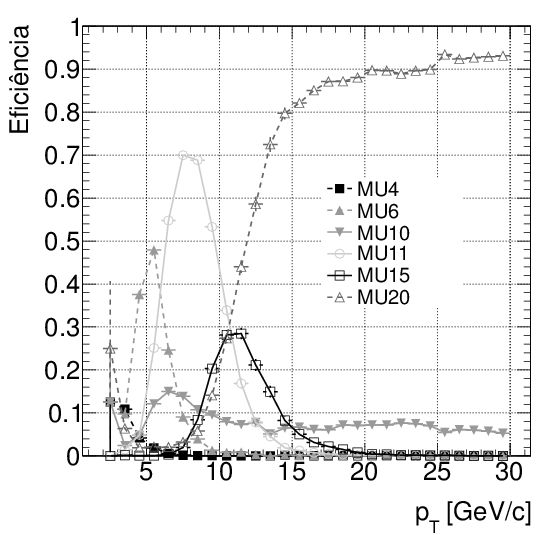
\includegraphics[width=12cm]{images/ppm_rpc_turnon_mu10.png}
    \caption{Eficiência de classificação do \emph{L1Muon} para eventos
    ocorridos no \emph{run} 191715.}
    \label{fig:muonrates}
\end{figure}

Pode-se observar que, como regra geral, a classificação obedece os patamares
preestabelecidos, ou seja, a distribuição de $p_T$ possui um pico em torno do
ponto de corte (por exemplo, 6~GeV para MU6) e final da calda antes do corte do
patamar seguinte. A única exceção é exatamente os eventos marcados como MU10,
cuja distribuição se prolonga até valores bastante elevados. Esse fato pode ser
explicado pelas áreas descobertas pelo terceiro plano RPC, por falhas no sistema
de alimentação do MS ou mesmo por múons, que mesmo com momento transverso
elevado, não conseguiram vencer o campo magnético toroidal.

Esse trabalho visa recuperar esses múons que foram classificados de maneira
equivocada. Para tal, foram projetados dois classificadores com objetivo
distintos com bases próprias:

\begin{enumerate}
    \item Classificador capaz de identificar se partículas marcadas como MU10 são
    realmente limitadas pelo patamar inferior de 10~GeV. Para esta análise, foram
    utilizados dados do \emph{run} 191715. São eventos datados de outubro de 2011. A
    configuração do detector previa a aquisição de múons independentes (eventos do
    tipo \emph{single muon} ou simplesmente \emph{sglmuon}). Eventos cujo $p_T >
    10$~GeV (totalizando 3518) são considerados alvo. Os restantes (365) são
    considerados falsos-alarmes.

    \item A etapa de  \emph{offline }classifica múons através de três critérios
    que variam de acordo com a acurácia desejada: \emph{tight}, \emph{medium} e
    \emph{loose}. O classificador projetado usou como alvo eventos aprovados
    pelo critério \emph{tight}. Eventos qualificados apenas no critério
    \emph{loose} foram considerados falsos-alarmes.  Neste projeto, foram
    utilizados dados de todos os \emph{2011} que foram configurados como
    \emph{minbias}. Nesta configuração, múons não são o principal objetivos,
    sendo assim, ruído de fundo do experimento. Usou-se essa configuração com
    intuito de isolar os efeitos do L1 em  relação ao classificador. Foram 2252
    eventos alvo contra
    430 indesejados.

\end{enumerate}

A Tabela~\ref{table:Classes} resume o número de eventos e a configuração
utilizada

\begin{table}[htbp!]
  \centering
  \begin{tabular}{ l  r  r  r  }
      \toprule
                         & Classe & Não-Classe & Configuração\\
      \midrule
        1 & 3518  & 365 & \emph{sglmuon} \\
        2 & 2252 & 430 &  \emph{minbias} \\ 
      \bottomrule
  \end{tabular}
  \caption{Resumo dos eventos MU10 considerados.}
  \label{table:Classes}

\end{table}



\section{Parâmetros de Avaliação do Desempenho}
\label{sec:performance_indexes}
A avaliação de eficiência dos algoritmos propostos nesse trabalho é realizada
através da utilização da curva ROC (\emph{Receiver Operating
Characteristic})~\cite{TREES2001} e pelo índice SP~\cite{ref:SIMAS}.

A curva ROC mostra como as probabilidades de detecção e falso alarme variam com
o patamar de decisão. A eficiência de um classificador pode ser estimada a
partir da área sob a curva ROC. Quanto maior a área, mais eficiente é o
discriminador~\cite{ref:SIMAS}.

O índice SP é definido por~\cite{CIODARO2012}:

\begin{equation}
SP = \sqrt{\sqrt{P_{\text{c}}P_{\text{nc}}} \left(\frac{P_{\text{c}} +
P_{\text{nc}}}{2}\right)}
\end{equation}

onde $P_\text{c}$ é a probabilidade de detecção da classe desejada e
$P_{\text{nc}}$ é a probabilidade de não obter um falso alarme.

O SP é  o parâmetro para escolher o patamar de decisão ótimo para um
classificador~\cite{ref:SIMAS}. Variando-se o patamar de decisão em toda sua
faixa de excursão , calculam-se os valores do SP correspondentes. O SP máximo
indica um patamar que apresenta alta eficiência para as duas classes.

\section{Metodologia}

Esta Seção apresenta a metodologia utilizada na tentativa de alcançar os
objetivos traçados anteriormente. Três abordagens foram realizadas: estudo da
deposição de energia de uma partícula passante na célula D do TileCal; utilizar
a geometria do detector ATLAS como fator classificatório e; projeto de
discriminadores neurais utilizando os parâmetros disponíveis no L1, confirmados
pela reconstrução \emph{offline} de múons.

\subsection*{Deposição de Energia}

Nesta abordagem, o histograma de distribuição da energia depositada pela
passagem de múons na camada externa do calorímetro hadrônico foi comparado com o
conjunto de falsos alarmes de cada um dos grupos descritos na
Seção~\ref{sec:data-section}.

Sabe-se que o ruído de fundo captado pelas células D possui média igual à 150
MeV e que a relação sinal-ruído é relativamente baixa, o que dificulta de a
utilização de patamares de energia~\cite{CIODARO2009}. Porém, há a possibilidade
de definir um patamar, acima do nível de ruído, capaz de aumentar a eficiência
de detecção, sem comprometer a taxa de eventos estabelecida para o L1, ou seja,
sem aumentar substancialmente a quantidade de falsos alarmes.

\subsection*{Casamento de Geometria}

Outra possibilidade é a utilização da geometria do calorímetro hadrônico e do
RPC. Como explicado, múons são elementos pesados e, portanto, sofrem pouca ação
dos campo magnéticos que atuam no ATLAS. Contudo, múons menos energéticos tendem
a ser desviados de modo mais acentuado. Ao dividir o ATLAS em setores azimutais
(setores de \emph{trigger}), em torno do ponto de interação, é possível
identificar quais partículas possuem trajetórias mais oblíquas.

O RPC é dividido logicamente em ROI, que são agrupadas em
setores de trigger. A informação de cada um desses setores, por sua vez, é
controlada por uma Sector Logic~(SL). Não há, porém, uma relação direta entra as
células D do calorímetro e uma RoI, devido a diferença de granularidade. Por sua
vez, um casamento entre o módulo do TileCal e o setor de trigger correspondente
é viável. Deste modo, todas as células D do detector são mapeadas nos setores de
\emph{trigger} do MS, de acordo com as suas posições $\phi$.

Nesta abordagem só são considerados múons de interesse os que cruzam um setor de
\emph{trigger}, quando combinadas com as informações geométricas da célula D.



\subsection*{Discriminador Neural}

As redes neurais artificiais~(RNA)~\cite{WASSERMAN1989,HAYKIN2008} são modelos
matemáticos inspirados em algumas características do cérebro humano, sendo
capazes de adquirir conhecimento e generalizar. Devido ao poder computacional,
obtido de sua estrutura paralelamente distribuído e suas habilidades, as RNAs
são usadas em diversas aplicações: reconhecimento de padrões~\cite{BISHOP1995},
controle e identificação de sistemas~\cite{ICHIKAWA1992}, processamento de
sinais~\cite{LAPEDES1987}, aproximação de funções~\cite{DENG2011}.

Uma diferença fundamental entre os classificadores neurais e os métodos
clássicos é que nestes últimos é necessário formular um modelo matemático a
partir dos sinais. Na abordagem neural, o classificador trabalha diretamente no
conjunto de dados, ficando o modelo matemático implícito nos valores dos pesos
sinápticos obtidos após o treinamento~\cite{ref:SIMAS}.

As redes de múltiplas camadas \emph{feed-forward} são compostas a partir da
formação sequencial de duas ou mais camadas de neurônios. A rede é composta por
três camadas: a entrada, a camada oculta e a saída. A camada oculta é
responsável por extrair características estatísticas de ordem elevada. Neste
trabalho foram utilizados sete neurônios na entrada e apenas um na saída. A
quantidade de neurônios da camada intermediária foi determinada mediante estudo
apresentado nas seções seguintes. A saída da rede foi projetada para resultar
$-1$ para eventos não desejados e $1$ para detecção. A Figura~\ref{fig:nnArch}
apresenta o modelo genérico de redes utilizados neste trabalho.

\begin{figure}[htbp!]
    \centering
    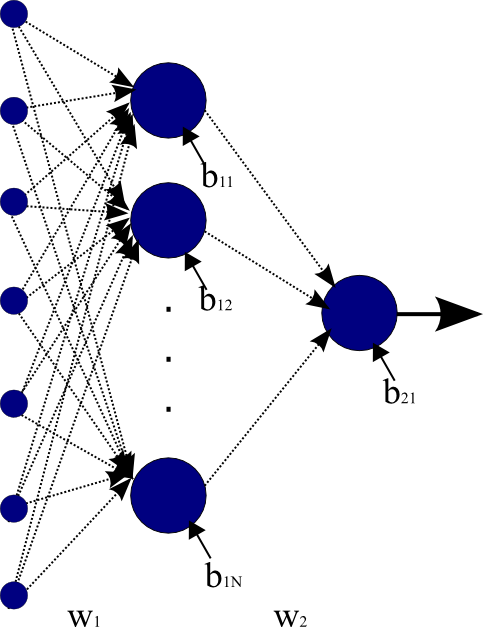
\includegraphics[height=6.5cm]{images/nnschema.png}
    \caption{Modelo de redes neurais utilizadas para discriminar os sinais de
    múons.}
    \label{fig:nnArch}
\end{figure}

As seguintes etapas foram realizadas para o projeto do discriminador neural.

\subsubsection{Robustez à Extrapolação em $\phi$ ($\phi$ \emph{Wrap-Around})}

As variáveis $\phi_\text{D}$ e $\phi_{\text{RoIRPC}}$ têm característica circular
e estão definidas no intervalo fechado ($-\pi$, $+\pi$). É possível ocorrerem
eventos onde, por exemplo, $\phi_\text{D}$ encontra-se próxima ao plano $\phi =
-\pi$ e a variável $\phi_{\text{RoIRPC}}$ esteja localizada no extremo oposto.
Para evitar esta distorção e manter a característica das variáveis em questão,
as seguintes transformações foram aplicadas:

\begin{eqnarray}
p^1 = \sin(\phi)\\
p^2 = \cos(\phi)
\end{eqnarray}

Deste modo, as variáveis $p^1_\text{D}$, $p^1_\text{RoIRPC}$,$p^2_\text{D}$,
$p^2_\text{RoIRPC}$ passam a ser utilizadas no treinamento, validação e operação
das redes neurais.

\subsubsection{Pré-processamento}

Para normalização a entrada e alvos da rede foram utilizadas a média e o desvio
padrão do conjunto de treino. Desta maneira, objetiva-se retirar a componente
média da amostra e deixar o desvio padrão unitário. Após o treinamento da rede,
os valores usados nesta normalização passam a fazer parte da rede, tanto quanto
as sinapses, devendo ser aplicados posteriormente no conjunto de teste e
validação.


\subsubsection{Especificação da Topologia}

Para decidir a quantidade de neurônios presentes na camada oculta, optou-se por
realizar uma série de treinos para 30 arquiteturas diferentes. Cada neurônio,
em todas as arquiteturas utilizadas, empregou a tangente hiperbólica como
função de ativação. A topologia que apresentar o maior valor médio para o índice
SP, considerando todas as rodadas utilizadas, foi considerada a melhor rede.

\subsubsection{Treinamento}

Os conjuntos utilizados foram separados de tal forma que 70\% dos eventos de
cada classe foram empregados para o desenvolvimento do pré-processamento e
treinamento. Mais 20\% foram separados para a análise do critério de
parada das redes empregadas. O restante serve para a validação pós-treino. Esse
procedimento será explicado mais adiante.

Os pesos foram inicializados utilizando valores aleatórios entre -0,2 e 0,2. O
treinamento utilizado foi o algoritmo \emph{Resilient
Backpropagation}~\cite{RIEDMILLER1993}. Ao final do treinamento, a rede neural
guardou as sinapses que proporcionaram o menor valor de MSE, de acordo com o
critério \emph{Save the Best}.

A Tabela~\ref{table:nnparameters} apresenta os valores utilizados para cada
parâmetro de treinamento.


\begin{table}[htbp!]\footnotesize
  \centering
  \tabcolsep=0.08cm
  \begin{tabular}{ m{7cm} m{3cm} }
      Parâmetro & Valor \\
      \midrule
      Figura de mérito           & MSE mínimo \\
      Número máximo de épocas    & 200.000 \\
      Gradiente mínimo           & $1e-10$ \\
      Taxa de aprendizagem       & 0.01 \\
      Mudança máxima de peso sinápticos    & 50\% \\
      Número máximo de falhas    & 1000 \\
      Número de inicializações   & 20 \\
      \bottomrule
  \end{tabular}
  \caption{Valores utilizados para cada parâmetro do treinamento neural.}
  \label{table:nnparameters}

\end{table}

\subsubsection{Análise da Flutuação Estatística}

Para que a flutuação estatística inerente aos dados empregados possa ser levada
em consideração na composição dos resultados, todos os discriminadores
desenvolvidos foram analisados através da validação cruzada~\cite{HAYKIN2008}.
Aqui, a validação foi realizada respeitando as seguintes etapas.

\begin{enumerate}
    \item Divide-se todo o conjunto em \emph{clusters} utilizando o algoritmo de
    \emph{K-Means}~\cite{HARTIGAN1979}. O número de agrupamentos é definido pelo
    índice de Davies--Bouldin~\cite{DAVIES1979}.
    \item Distribuem-se os \emph{clusters} igualmente entre 10 blocos. Desta
    maneira, espera-se que cada bloco possua características estatísticas
    similares entre si. Além disso, cada bloco constitui uma representação em
    menor escala do conjunto todo.
    \item Sete blocos são separados para o conjunto, dois blocos para validação
    e um para teste.
    \item O discriminador neural é treinado.
    \item Os resultados obtidos são armazenados
    \item Os últimos três passos são então repetidos nove vezes variando a
    seleção de blocos, e nunca repetindo aquele já selecionado para o conjunto
    de teste em um treinamento anterior para a mesma função.
\end{enumerate}


%%%%%%%%%%%%%%%%%
%%%
%%% Resultados
%%%%%%%%%%%%%%%%%%

\chapter{Resultados e Discussão}

Neste capítulo, são apresentados os resultados obtidos ao aplicar a metodologia
indicada no capítulo anterior. Os dados utilizados foram obtidos em colisões
observadas no ATLAS, em 2011, cuja energia total foi igual a 7~GeV.

Foram utilizadas as informações relativas a geometria da célula D do TileCal
($\phi$ e $\eta$) e do MS ($\phi$ e $\eta$) para um evento de múon.  A energia
($E_\text{D}$) depositada pela passagem da partícula na célula do calorímetro também
foi levada em consideração.

Foram projetados dois classificadores com objetivos distintos com bases
próprias. O primeiro é capaz de identificar se partículas marcadas como MU10
são realmente limitadas pelo patamar inferior de 10~GeV. Para esta análise,
foram utilizados dados do \emph{run} 191715. O segundo usou como alvo eventos
aprovados pelo critério \emph{tight}. Eventos qualificados apenas no critério
\emph{loose} foram considerados falsos-alarmes.  Aqui, foram utilizados dados
de todos os  \emph{runs} de 2011 que foram configurados como \emph{minbias}.


\section{Discriminação de múons de alto $p_T$ e baixo $p_T$}

Existe uma região de confusão entre múons de alto e de baixo momento
transverso, em torno de 10~GeV. Essa característica faz com que uma parte dos
múons de alto momento transverso sejam sempre identificados pelo patamar MU10,
sensível aos múons de baixo $p_T$. Assim, esse patamar opera com um elevado
prescale, o que diminui a quantidade de múons de alto momento transverso
observados.

Nesta etapa, procurou-se verificar se a célula D serviria como substituta da
camada do RPC faltante. Uma terceira etapa de coincidência deixa a aquisição
menos sensível a múons de baixo $p_T$, aumentando a a probabilidade de detectar
múons de alta energia corretamente.


\subsection*{Deposição de Energia}

O histograma da distribuição de energia depositada pela passagem de múons de
alto $p_T$ na célula D foi comparado com o conjunto de múons de baixo $p_T$.
Todos foram classificados no \emph{online} como MU10, e seus respectivos
momentos foram estimados pelo \emph{offline}. Na
Figura~\ref{fig:histEnergy191715}, pode-se verificar que as duas distribuições
são muito similares, o que dificulta a determinação de um patamar que possa ser
aplicado aos sinais e atue como um discriminador. Outro detalhe visível é  a
distância das duas distribuições em relação ao ruído eletrônico (ou
\emph{pedestal}).

\begin{figure}[htpb!]
    \centering
    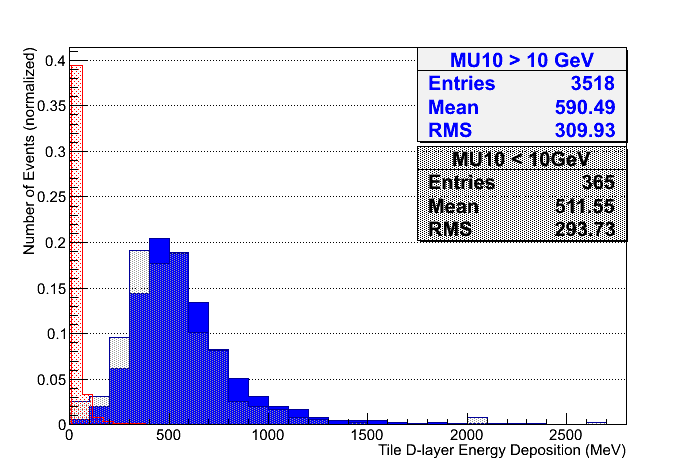
\includegraphics[width=10cm]{images/sglmuon/histEnergyDeposition.png}
    \caption{Distribuição da energia depositada na célula D do TileCal durante o
    \emph{run} 191715. Em azul, os múons com $p_T >$ 10~GeV. Em cinza, os múons
    com $p_T <$ 10~GeV. Em vermelho, a distribuição do ruído eletrônico.}
    \label{fig:histEnergy191715}
\end{figure}

Como pode-se observar na Figura~\ref{fig:ROCEnergy191715}, a eficiência de
detecção para as duas classes é muito semelhante. A curvatura da curva ROC é
muito sutil. O ponto de SP máximo dá-se quando o patamar de corte é igual a
500~MeV, onde a taxa detecção chega a aproximadamente 60\% e o falso-alarme
fica acima de 50\%.

Percebe-se assim que um corte por patamar de energia sozinho não é suficiente
para distinguir a classe alvo.

\begin{figure}[H]
        \centering
        \begin{subfigure}[b]{0.45\textwidth}
                \centering
                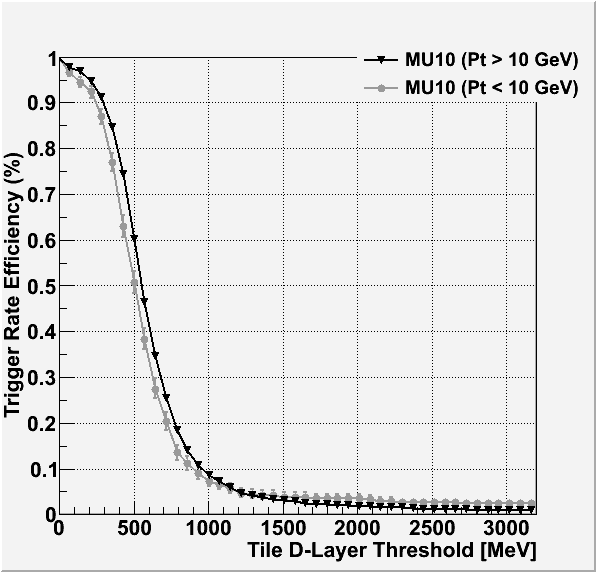
\includegraphics[width=\textwidth]{images/sglmuon/roc_nomatch.png}
        \end{subfigure}%
        ~
        \begin{subfigure}[b]{0.45\textwidth}
                \centering
                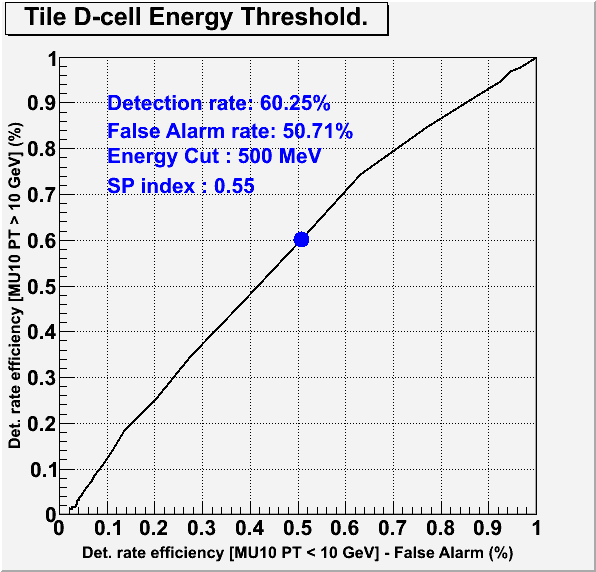
\includegraphics[width=\textwidth]{images/sglmuon/roc_perf_nomatch.png}
        \end{subfigure}
        \caption{Curva ROC para o uso de patamar de energia.}
        \label{fig:ROCEnergy191715}
\end{figure}



\subsection*{Casamento de Geometria}

A Figura~\ref{crossgeo} procura mostrar o quão oblíquo é a trajetória dos múons
que cruzaram o TileCal e o RPC durante o \emph{run} escolhido. No eixo $x$,
encontramos a diferença em $\eta$ entre os pontos de cruzamentos na célula D e
no RoI do RPC. A escala de cor representa a quantidade de eventos que obtiveram
a mesma inclinação. O histograma superior apresenta os eventos com baixo $p_T$ e
o inferior com alto $p_T$. Pode-se notar que a distribuição do primeiro é mais
dispersa, principalmente em $\phi$. Este comportamento deve-se ao fato de múons
menos energéticos tendem a ser desviados de modo mais acentuado.

\begin{figure}[htpb!]
    \centering
    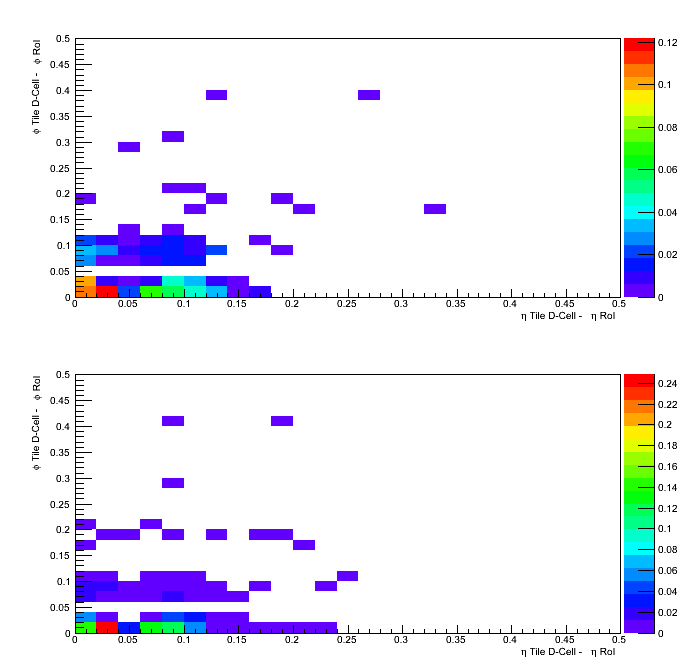
\includegraphics[width=11cm]{images/sglmuon/crossGeo.png}
    \caption{Histograma apresentando o quão oblíqua é a trajetória do múon. O
    primeiro gráfico representa os eventos com partículas com baixo momento
    transverso e o segundo com alto.}
    \label{crossgeo}
\end{figure}

É estabelecer um novo patamar de corte ao rejeitar todas as partículas que
atravessem  setores de \emph{trigger} distintos. Para tal, as células D do
detector são mapeadas, de acordo com as suas posições $\phi$, em relação aos
setores do espectrômetro.

A partir da Figura~\ref{fig:ROCSL191715} conclui-se que, apesar de excluir
partículas também do conjunto alvo, casando as geometrias dos dois detectores há
uma melhora na taxa de detecção. A curva ROC possui um ângulo de inclinação mais
acentuado em relação à curva apresentada anteriormente. O corte em energia passa
a ser aproximadamente 430~MeV. Desta forma, observa-se que considerar as
características geométricas do detector é interessante para a classificação.

\begin{figure}[htpb!]
        \centering
        \begin{subfigure}[b]{0.45\textwidth}
                \centering
                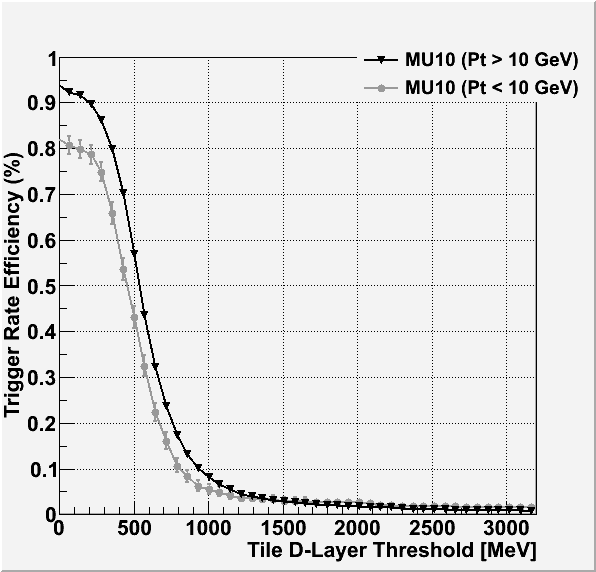
\includegraphics[width=\textwidth]{images/sglmuon/roc_match_SL.png}
        \end{subfigure}%
        ~
        \begin{subfigure}[b]{0.45\textwidth}
                \centering
                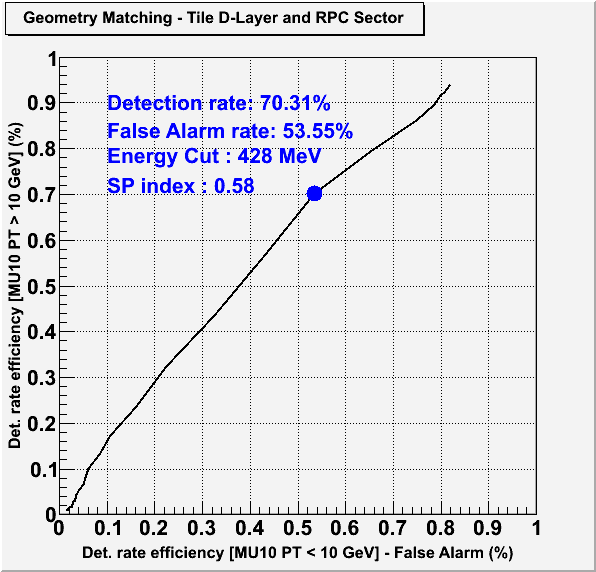
\includegraphics[width=\textwidth]{images/sglmuon/roc_perf_match_SL.png}
        \end{subfigure}
        \caption{Curva ROC para o uso de patamar de energia ao casar as
        geometrias do TileCal e do RPC.}
        \label{fig:ROCSL191715}
\end{figure}


\subsection*{Discriminador Neural}

A primeira etapa no projeto do discriminador neural foi separar os dados em
conjuntos de treino, teste e validação. Para a realização dos treinos, foi
escolhida como metodologia a validação cruzada, a fim de minimizar os efeitos da
flutuação estatísticas. Com ela, espera-se a obtenção de uma topologia ótima
para o problema.

Primeiramente, agrupou-se as amostras para evidenciar eventos com
características estatísticas semelhantes. O índice de Davies-Bouldin determinou
22 \emph{clusters} como ideal para o conjunto apresentado. O algoritmo
\emph{K-Means} foi utilizado para a tarefa. A Figura~\ref{fig:clusters191715}
mostra o resultado da divisão em agrupamentos. Interessante perceber que nenhum
dos \emph{clusters} formados evidenciou uma das classes.

\begin{figure}[htpb!]
    \centering
    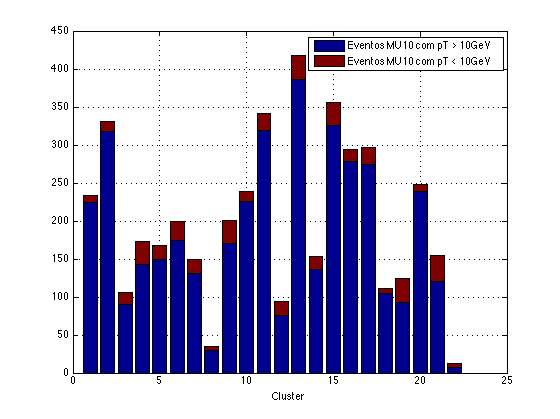
\includegraphics[width=11cm]{images/sglmuon/distribuicao_clusters.png}
    \caption{Eventos de múon separados em 22 \emph{clusters} depois de aplicado
    o algoritmo de \emph{K-means}. Em vermelho, estão representados os múons de
    baixo $p_T$. Em azul, os múons de alto $p_T$.}
    \label{fig:clusters191715}
\end{figure}

Os dados dos \emph{clusters} foram igualmente distribuídos entre 10 os blocos.
Desta maneira, espera-se que cada bloco possua características estatísticas
similares entre si.  As Figuras~\ref{fig:bloco191715-1}, \ref{fig:bloco191715-2} e
\ref{fig:bloco191715-3} mostram os dados distribuídos nos blocos. Neste ponto,
as informações sobre múons de baixo $p_T$ são replicadas em cada um dos blocos,
de forma que a representatividade das duas classes seja parelha.


\begin{sidewaysfigure}
    \centering
    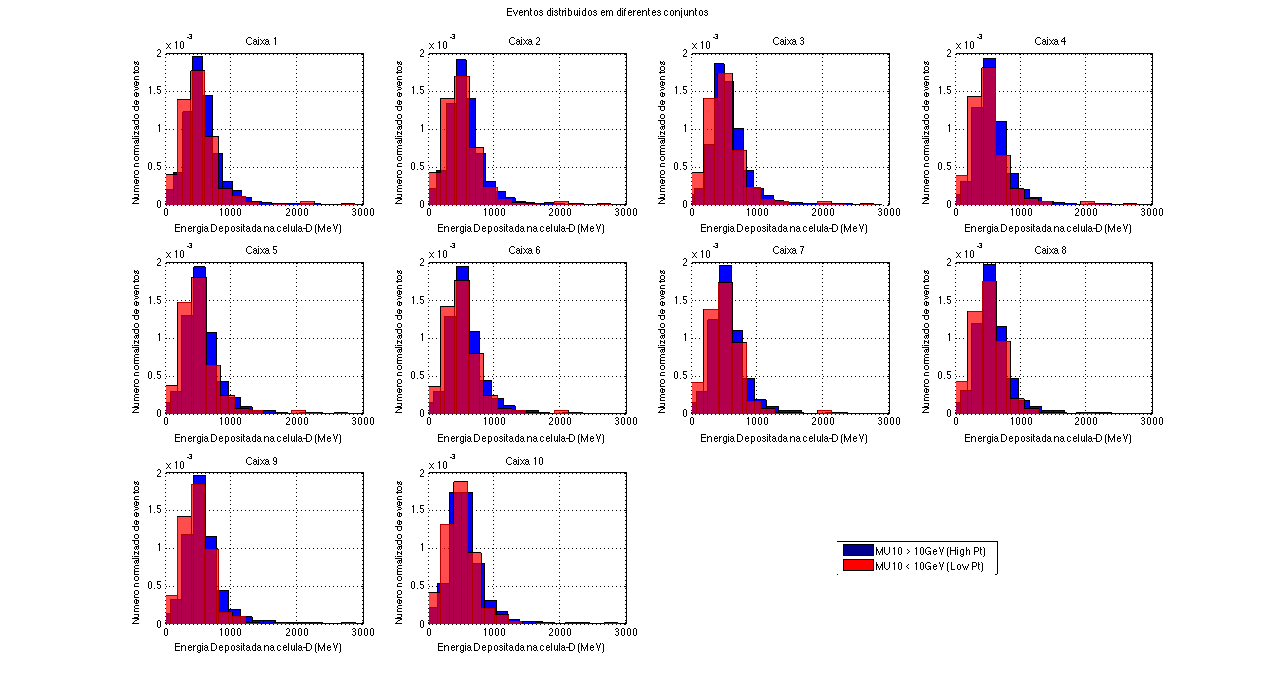
\includegraphics[width=\textheight]{images/sglmuon/eventos_caixas.png}
    \caption{Eventos de múons divididos em 10 blocos. As distribuições da
    energia depositada na célula D. Os histogramas dos diferentes blocos devem
    ser semelhantes.}
    \label{fig:bloco191715-1}
\end{sidewaysfigure}

\begin{sidewaysfigure}
    \centering
    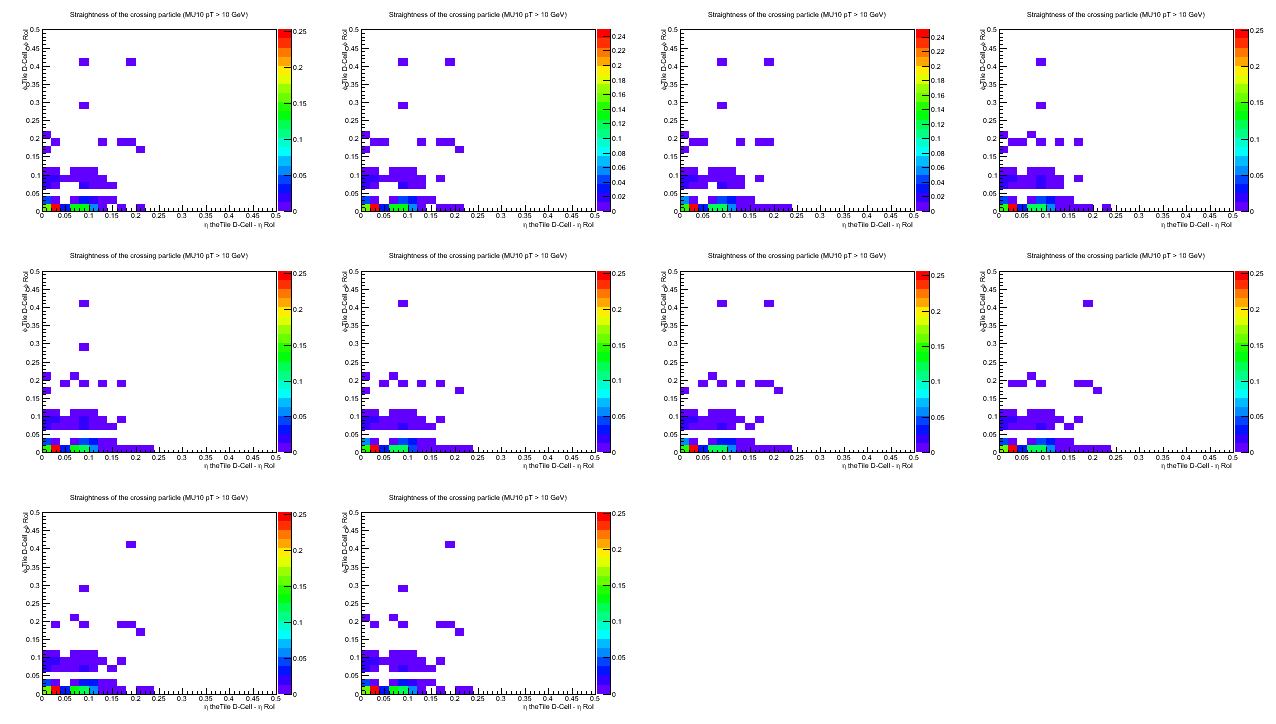
\includegraphics[width=\textheight]{images/sglmuon/cluster_eta_phi_class.png}
    \caption{Eventos de múons divididos em 10 blocos. \emph{Hits} na camada D do
    TileCal e nas regiões de interesse do RPC. Aqui estão representados os
    eventos de alto $p_T$}
    \label{fig:bloco191715-2}
\end{sidewaysfigure}

\begin{sidewaysfigure}
    \centering
    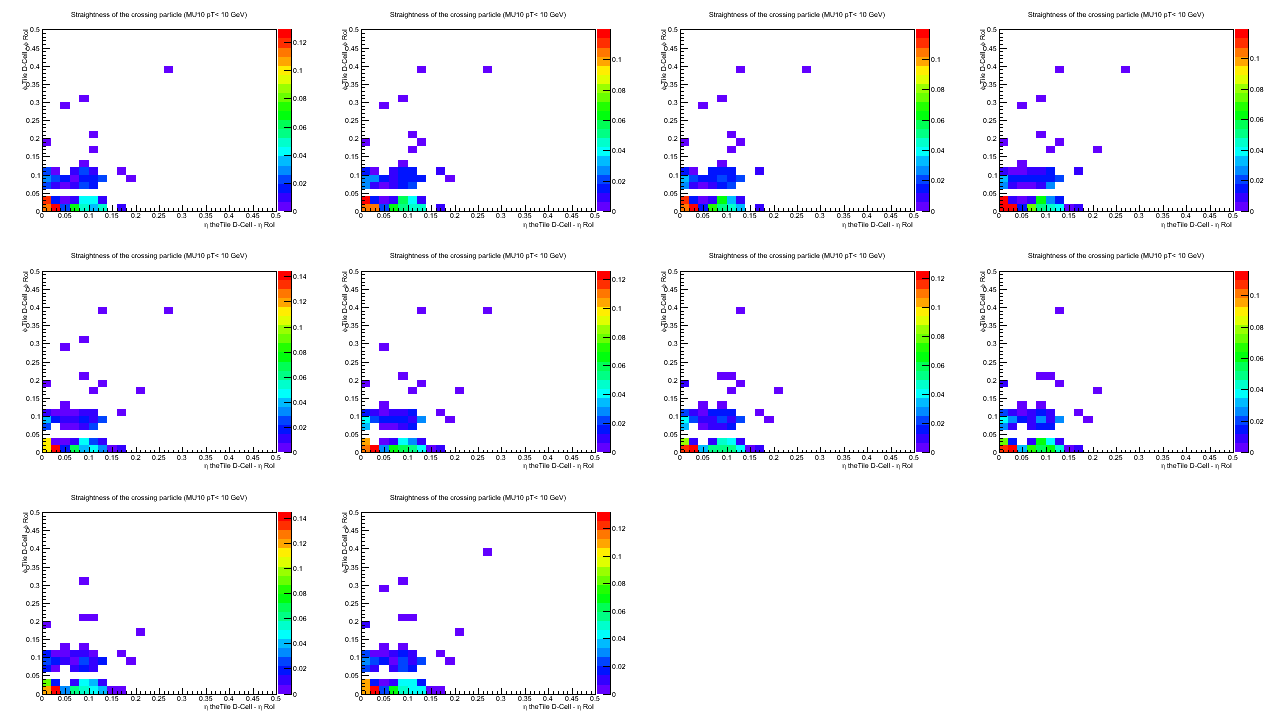
\includegraphics[width=\textheight]{images/sglmuon/cluster_eta_phi_noclass.png}
    \caption{Eventos de múons divididos em 10 blocos. \emph{Hits} na camada D do
    TileCal e nas regiões de interesse do RPC. Aqui estão representados os
    eventos de baixo $p_T$}
    \label{fig:bloco191715-3}
\end{sidewaysfigure}

Ao todo, 31 topologias foram treinadas. Por sua vez, cada uma foi treinada com
10 arranjos diferentes de treino, teste e validação. Cada rede foi inicializada
20 vezes com intuito de evitar mínimos locais e a que tiver melhor índice de SP
para o conjunto de validação será armazenada. No total, foram realizadas 6.200
rodadas de treino para selecionar a topologia ideal. 

A Figura~\ref{fig:Topology191715} mostra o índice de SP médio para cada
topologia treinada, levando em consideração os 10 blocos utilizados. No gráfico,
ainda é possível verificar o valor máximo e mínimo conseguido. A incerteza é
representada pelo desvio padrão. Levando em consideração o SP mais elevado, a
rede com 15 neurônios na camada escondida foi escolhida.

A Figura~\ref{fig:ROCNN191715} apresenta a  curva ROC para a rede com 15
neurônios na camada intermediária que obteve maior valor de SP. Observa-se que
ela obteve um ganho de 5\% em detecção em relação à proposta de casamento de
geometria.  Referente à taxa de falso-alarme, a rede proporcionou um grande
ganho, reduzindo-o para aproximadamente 15\%.


\begin{figure}[htpb!]
    \centering
        \begin{subfigure}[b]{0.45\textwidth}
                \centering
            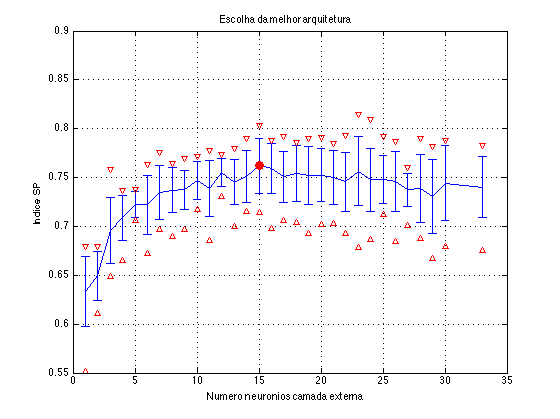
\includegraphics[width=\textwidth]{images/sglmuon/plotSP.png}
            \caption{Escolha da melhor Topologia. Com base nesse gráfico podemos
            perceber que a topologia com 15 neurônios obteve melhor desempenho.}
            \label{fig:Topology191715}
        \end{subfigure}%
        ~
        \begin{subfigure}[b]{0.45\textwidth}
                \centering
                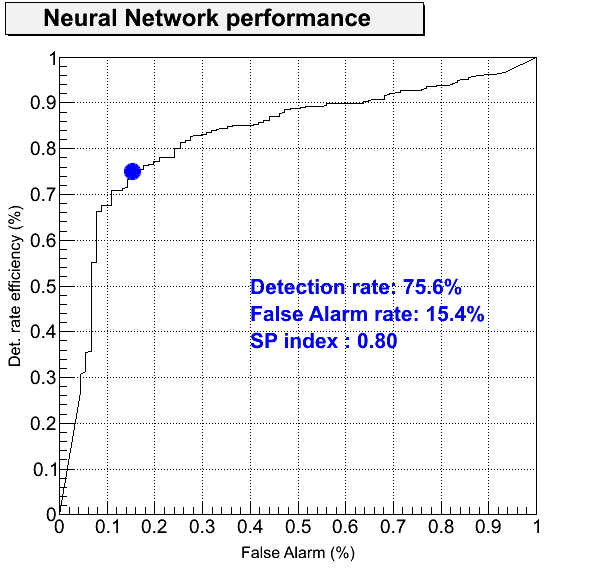
\includegraphics[width=\textwidth]{images/sglmuon/roc_perf_match_NN.png}
            \caption{Curva ROC para saída da rede neural com 15 neurônios na
            camada escondida.}
            \label{fig:ROCNN191715}
        \end{subfigure}
        \caption{Projeto de discriminador neural.}
\end{figure}

\section{Discriminação de múons verdadeiros e falsos.}

Como podemos notar pela Figura~\ref{fig:rejected} existe um grande número de
múons que são detectados pelo L1, mas posteriormente descartados pelos
algoritmos \emph{offline}.


\begin{figure}[htp!]
   \centering
   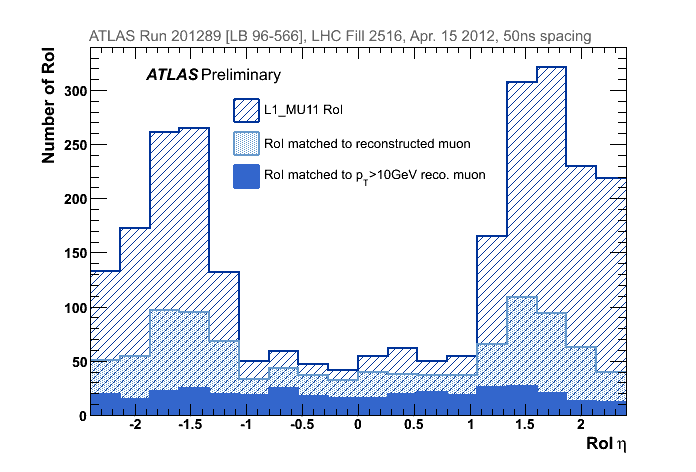
\includegraphics[width=11cm]{images/muon_rejected.png}
   \caption[Distribuição de RoI em $\eta$ com múons aprovados. É mostrado qual
   percentual é confirmado posteriormente pelos algoritmos \emph{offline} ]%
   {Distribuição de RoI em $\eta$ com múons aprovados. É mostrado qual
   percentual é confirmado posteriormente pelos algoritmos \emph{offline}
   (Retirado de~\cite{BUTTINGER2012}).}
   \label{fig:rejected}
\end{figure}
%%%

Nesta etapa, procurou-se verificar se a informação da  célula D ajudaria a
identificar falsos múons e assim, melhorar a eficiência do sistema de aquisição.


\subsection*{Deposição de Energia}


O histograma da distribuição de energia depositada pela passagem de múons
(partículas aprovadas pelo critério \emph{tight}) na célula D foi comparado com
o conjunto de falsos múons (rejeitados pelo \emph{tight}, mas, no caso,
aprovados pelo \emph{loose}).  Todos foram classificados no \emph{online} como
MU10, e seus respectivos momentos foram estimados pelo \emph{offline}. Na
Figura~\ref{fig:histEnergyminbias}, pode-se verificar que, como no caso
anterior,  as duas distribuições são muito similares.


\begin{figure}[htpb!]
    \centering
    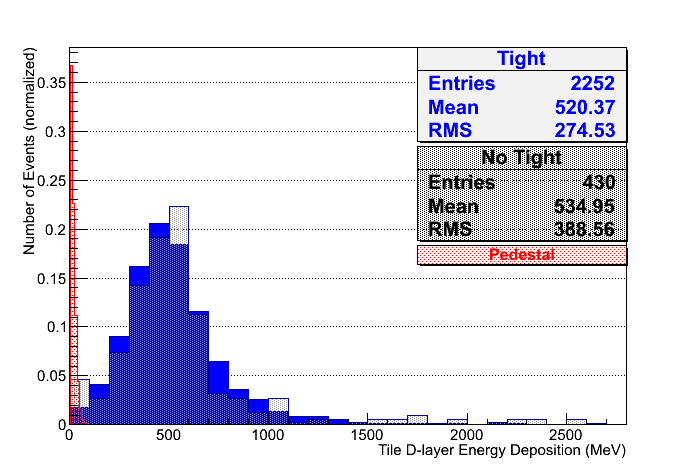
\includegraphics[width=12cm]{images/minbias/histEnergyDeposition.png}
    \caption{Distribuição da energia depositada na célula D do TileCal para
    todos os \emph{runs} de 2011 com configuração de \emph{minbias}.}
    \label{fig:histEnergyminbias}
\end{figure}


Como pode-se observar na Figura~\ref{fig:ROCEnergyminbias}, a eficiência de
detecção para as duas classes é muito semelhante. O coeficiente linear da curva
é unitário, ou seja, apenas a informação de energia é insuficiente para tarefa.
O ponto de SP máximo dá-se quando o patamar de corte é igual a 567~MeV, onde a
taxa detecção e o falso-alarme possuem taxas  aproximadamente 62\%.

\begin{figure}[htpb!]
        \centering
        \begin{subfigure}[b]{0.45\textwidth}
                \centering
                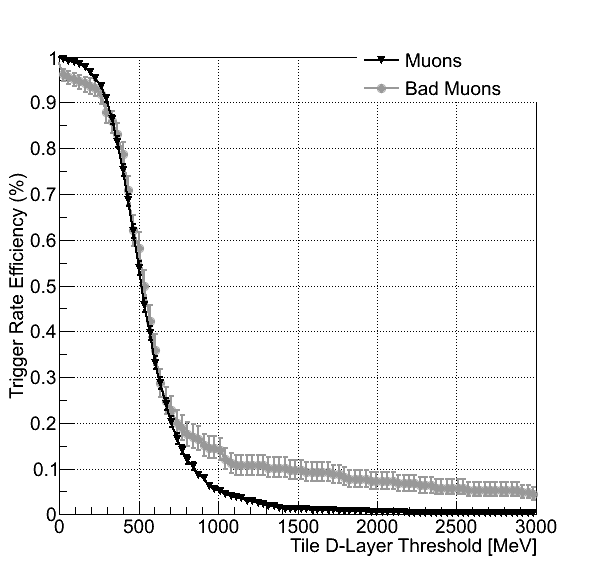
\includegraphics[width=\textwidth]{images/minbias/C.png}
        \end{subfigure}%
        ~
        \begin{subfigure}[b]{0.45\textwidth}
                \centering
                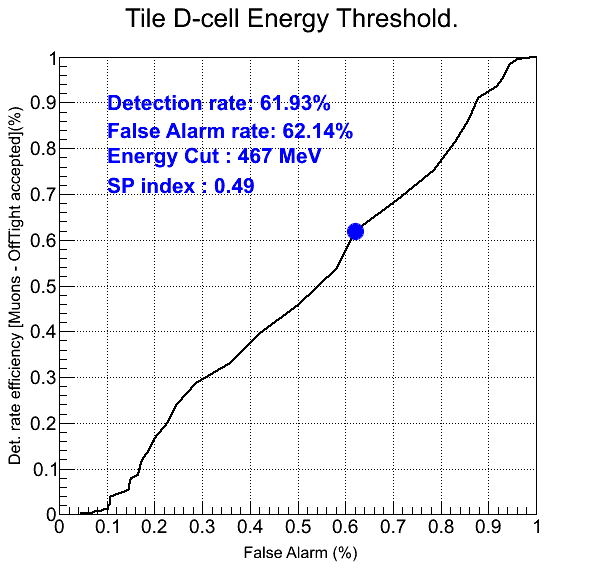
\includegraphics[width=\textwidth]{images/minbias/C_roc.png}
        \end{subfigure}
        \caption{Curva ROC ao considerar patamares de energia}
        \label{fig:ROCEnergyminbias}
\end{figure}G

\subsection*{Casamento de Geometria}

A Figura~\ref{crossgeominbias} procura mostrar o quão oblíquo é a trajetória dos múons
que cruzaram o TileCal e o RPC durante o \emph{run} escolhido. No eixo $x$,
encontramos a diferença em $\eta$ entre os pontos de cruzamentos na célula D e
no RoI do RPC. A escala de cor representa a quantidade de eventos que obtiveram
a mesma inclinação.

Pode-se notar que a distribuição do primeiro é mais dispersa, principalmente em
$\phi$. Nesse caso, existem algumas possibilidades como, por exemplo, o fato de
múons provenientes de pontos diferentes ao ponto de interação (raios cósmicos)
traçam trajetórias que não são necessariamente normais ao plano do tubo do LHC
ou mesmo partículas mais leves que acabaram cruzando o MS. De qualquer maneira,
o casamento geométrico pode ser utilizado para maximizar a detecção dos
verdadeiros múons.

A Figura~\ref{fig:ROCSLminbias} mostra que casando as geometrias dos dois
detectores há uma redução na taxa de falso-alarme de 5\%. O índice SP igual a
0.52 mostra que, apesar da redução, a medida não foi suficiente para realizar a
discriminação.

\begin{figure}[htpb!]
    \centering
    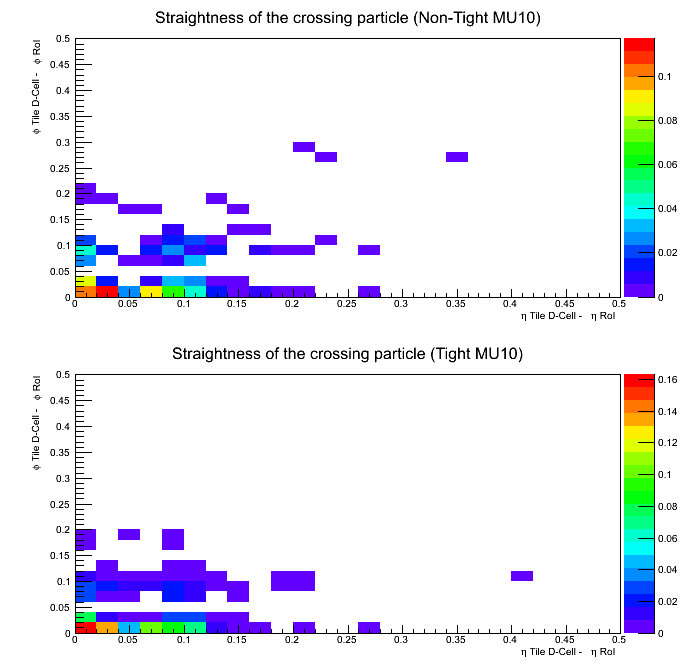
\includegraphics[width=11cm]{images/minbias/crossGeo.png}
    \caption{Histograma apresentando o quão oblíqua é a trajetória do múon. O
    primeiro gráfico representa os eventos com partículas não confirmadas pelo
    critério \emph{tight}, enquanto no segundo apenas confirmadas.}
    \label{crossgeominbias}
\end{figure}

\begin{figure}[htpb!]
        \centering
        \begin{subfigure}[b]{0.45\textwidth}
                \centering
                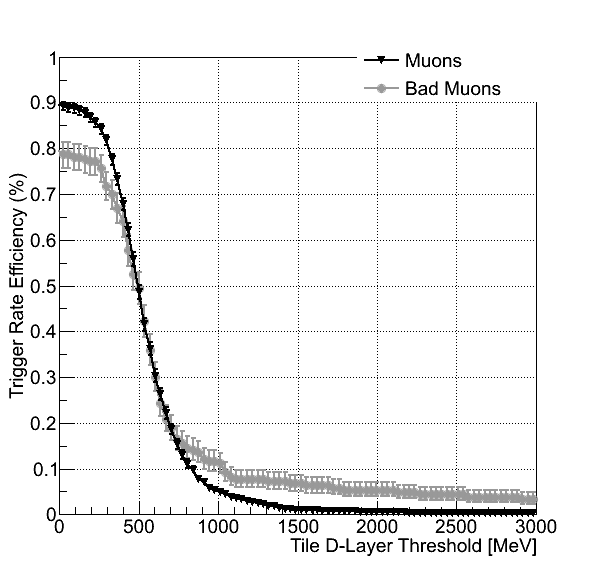
\includegraphics[width=\textwidth]{images/minbias/C_match.png}
        \end{subfigure}%
        ~
        \begin{subfigure}[b]{0.45\textwidth}
                \centering
                \includegraphics[width=\textwidth]{images/minbias/C_roc_match.png}
        \end{subfigure}
        \caption{Curva ROC para o uso de patamar de energia ao casar as
        geometrias do TileCal e do RPC.}
        \label{fig:ROCSLminbias}
\end{figure}


\subsection*{Discriminador Neural}

Foi novamente escolhida a metodologia de validação cruzada para o projeto do
discriminador neural. Primeiramente, as amostras foram agrupadas em 9
\emph{clusters}. O número de \emph{clusters} utilizado foi determinado pelo
índice de Davies-Bouldin. A Figura~\ref{fig:clustersminbias} mostra o resultado da
divisão em agrupamentos. Mais uma vez, nenhum dos \emph{clusters} formados
evidenciou uma das classes.

\begin{figure}[htpb!]
    \centering
    \includegraphics[width=11cm]{images/minbias/kmeans_cluster.png}
    \caption{Eventos de múon separados em 9 \emph{clusters} depois de aplicado
    o algoritmo de \emph{K-means}.}
    \label{fig:clustersminbias}
\end{figure}

Os dados dos \emph{clusters} foram igualmente distribuídos entre 10 os blocos.
As Figuras~\ref{fig:blocominbias-1}, \ref{fig:blocominbias-2} e
\ref{fig:blocominbias-3} mostram os dados distribuídos nos blocos. Neste ponto,
as informações sobre múons falsos são replicadas em cada um dos blocos, de forma
que a representatividade das duas classes seja parelha.


\begin{sidewaysfigure}
    \centering
    \includegraphics[width=\textheight]{images/minbias/histClusters.png}
    \caption{Eventos de múons divididos em 10 blocos. As distribuições da
    energia depositada na célula D. Os histogramas dos diferentes blocos devem
    ser semelhantes.}
    \label{fig:blocominbias-1}
\end{sidewaysfigure}

\begin{sidewaysfigure}
    \centering
    \includegraphics[width=\textheight]{images/minbias/cluster_phi_eta_class.png}
    \caption{Eventos de múons divididos em 10 blocos. \emph{Hits} na camada D do
    TileCal e nas regiões de interesse do RPC. Todos eventos aprovados pelo
    critério \emph{tight}.}
    \label{fig:blocominbias-2}
\end{sidewaysfigure}

\begin{sidewaysfigure}
    \centering
    \includegraphics[width=\textheight]{images/minbias/cluster_phi_eta_noclass.png}
    \caption{Eventos de múons divididos em 10 blocos. \emph{Hits} na camada D do
    TileCal e nas regiões de interesse do RPC. Todos eventos reprovados pelo
    critério \emph{tight}.}
    \label{fig:blocominbias-3}
\end{sidewaysfigure}

Ao todo, 30 topologias foram treinadas. Por sua vez, cada uma foi treinada com
10 arranjos diferentes de treino, teste e validação. Cada rede foi inicializada
20 vezes com intuito de evitar mínimos locais e a que tiver melhor índice de SP
para o conjunto de validação será armazenada. No total, foram realizadas 6.000
rodadas de treino para selecionar a topologia ideal.

A Figura~\ref{fig:Topologyminbias} mostra o índice de SP médio para cada
topologia treinada, levando em consideração os 10 blocos utilizados. No gráfico,
ainda é possível verificar o valor máximo e mínimo conseguido. A incerteza é
representada pelo desvio padrão. Levando em consideração o SP mais elevado, a
rede com 29 neurônios na camada escondida foi escolhida.

A Figura~\ref{fig:ROCNNminbias} apresenta a  curva ROC para a rede com 29
neurônios na camada intermediária que obteve maior valor SP para o conjunto de
validação de dados. Neste caso, observou-se um grande aumento de performance. A
taxa de detecção aumenta cerca de 20\% em relação aos outros métodos utilizados
e o falso-alarme é reduzido a 40\%.

\begin{figure}[htpb!]
    \centering
        \begin{subfigure}[b]{0.45\textwidth}
                \centering
            \includegraphics[width=\textwidth]{images/minbias/plotSP.png}
            \caption{Escolha da melhor Topologia. Com base nesse gráfico podemos
            perceber que a topologia com 29 neurônios na camada oculta obteve
            melhor desempenho.}
            \label{fig:Topologyminbias}
        \end{subfigure}%
        ~
        \begin{subfigure}[b]{0.45\textwidth}
                \centering
                \includegraphics[width=\textwidth]{images/minbias/C_roc_nn.png}
            \caption{Curva ROC para saída da rede neural com 29 neurônios na
            camada oculta.}
            \label{fig:ROCNNminbias}
        \end{subfigure}
        \caption{Projeto de discriminador neural.}
\end{figure}


  \chapter{Conclusões}

A identificação de múons de todos os patamares energéticos é crucial para
explorar todo potencial físico disponível através da operação do ATLAS. A partir
da observação destas partículas é possível conhecer novas físicas.

O Espectrômetro de Múons é instalado na camada externa do ATLAS e foi projetado
para detectar essas partículas. A estratégia deste sistema é aplicar um campo
magnético intenso, capaz de curvar a trajetória da partícula. Ao detectar a
passagem do alvo por suas três estações, o experimento consegue traçar o
caminho percorrido e, como consequência, estimar o momento transverso da
partícula. Contudo, há regiões onde não há cobertura de câmaras nas três
camadas. Nestas áreas todos os múons são classificados automaticamente como
pouco energéticos, prejudicando a eficiência de detecção.

Esta dissertação procurou recuperar os múons de momento elevado utilizando
informações geométricas do calorímetro e do sistema de múons, somadas à energia
depositada pela passagem de partículas na célula D. Esta célula localiza-se na
camada externa do TileCal e possui, portanto, baixa atividade hadrônica. Deste
modo, suas informações podem ser utilizadas para ajudar na detecção de múons.
Este trabalho é o desdobramento de~\cite{CIODARO2010}, que forneceu o estudo e
propôs um sistema capaz de melhorar a detecção de múons utilizando informações
de calorimetria. Este trabalho também apresentou uma metodologia para avaliar a
resposta do RPC à radiação de fundo da caverna do ATLAS.

Durante o desenvolvimento deste projeto, foram realizadas diversas reuniões com
a colaboração, o que possibilitou o melhor entendimento em relação ao sistema de
filtragem do L1, à seleção de múons e ao sistema de calorimetria. Também foram
disponibilizados dados de colisão ocorridos em 2011, o que viabilizou a
execução.

O Capítulo 4 apresentou inicialmente a metodologia utilizada durante o projeto.
Três abordagens foram realizadas:  estudo da deposição de energia de uma
partícula passante na célula D do TileCal; utilização da geometria do detector
ATLAS como fator classificatório; projeto de discriminadores neurais
utilizando os parâmetros disponíveis no L1, confirmados pela reconstrução
\emph{offline} de múons.

Através dos resultados pode-se observar que o depósito de energia na célula é
muito semelhante para todas as distribuições estudadas. A alta taxa de falso
alarme inviabiliza a utilização técnica de corte por patamar de energia sozinha.
Quando utilizou-se as informações de geometria do calorímetro logicamente
casadas à posição das regiões de interesse do RPC, obteve-se um pequeno ganho na
detecção, aliado à redução da taxa de falso alarme.

A utilização de classificadores neurais mitigou a taxa de falso alarme para
patamares condizentes com os requisitos de operação do L1. A taxa de detecção
obtida em ambos os conjuntos estudados indica que a célula D pode vir a ser uma
possível substituta da camada ausente do RPC. A Tabela~\ref{summary}
resume todos os resultados apresentados no Capítulo~5.

\begin{table}[hptp!]\footnotesize
  \centering
  \tabcolsep=0.08cm
  \begin{tabular}{ r c c c c c c }
       \multicolumn{1}{c}{} & \multicolumn{3}{c}{Detecção MU10}& \multicolumn{3}{c}{Detecção Múons Verdadeiros} \\
        \cmidrule(r){2-4}
        \cmidrule(r){5-7}
      & Dep. Energia & Geometria & Rede Neural & Dep. Energia & Geometria & Rede Neural \\
      \midrule
      Prob. Detecção & 60,3\% & 70,3\% & 75,6\% & 61,9\%  & 62,2\% & 82,3\% \\[1.5ex]
      Falso Alarme   & 50,7\% & 53,6\% & 15,4\% & 62,1\%  & 57,8\% & 21,2\% \\[1.5ex]
      Indice SP      & 0,55   & 0,58   & 0,80 & 0,49    & 0,51   & 0.82   \\
      \bottomrule
  \end{tabular}
  \caption{Tabela resumindo os resultados obtidos neste trabalho.}
  \label{summary}
\end{table}



À luz do \emph{upgrade} do detector, previsto para a operação em 2020, com
etapas intermediárias em 2013 e 2017, novas arquiteturas podem ser propostas. O
projeto e implantação de uma placa eletrônica que implemente as redes neurais
propostas nesse estudo no L1 é um dos desdobramentos possíveis. Antes, porém,
seria interessante um estudo mais detalhado da resposta do sistema proposto
frente à radiação de fundo do ATLAS.

  \end{spacing}



  \backmatter
  \bibliographystyle{coppe-unsrt}
  \bibliography{thesis}

 % \appendix
 % \include{appenA}
\end{document}
